\section{Verification}
\label{section: Chapter5/verification}

Unless otherwise stated, we choose $C = \beta$ for the modified fracture energy \eqref{eq: modified fracture energy} and the fracture dual kinetic potential\eqref{eq: fracture dual kinetic potential} to satisfy the second law of thermodynamics. All other model parameters and material constants are provided separately for each of the problems in this section, below.

\begin{figure}[htb!]
  \centering
  \begin{subfigure}{0.4\textwidth}
    \centering
    \tikzsetnextfilenamesafe{Chapter5/terminology/EPD}
    \begin{tikzpicture}
      \begin{axis}[
          width=\textwidth,
          height=\textwidth,
          xmin=0,
          xmax=0.06,
          ymin=0,
          ymax=370,
          xlabel=total strain,ylabel=stress,
          xtick={0.016,0.0273645},
          xticklabels={$\varepsilon^p_c$,$\varepsilon_c$},
          ytick={320,346},
          yticklabels={$\sigma_y$,$\sigma_c$},
          scaled x ticks=false
        ]
        \addplot +[thick,mark=none,black] table[x=total_strain,y=stress,col sep=comma]{Chapter5/data/terminology.csv};
        \path [name path=f] (0.016,0) -- (0.0273645,346);
        \path [name path=axis] (axis cs:0,0) -- (axis cs:1,0);
        \addplot [thick,color=blue,fill=blue,fill opacity=0.2] fill between[of=f and axis,soft clip={domain=0:0.0273645}];
        \draw [dashed, thick] (0,320) -- (0.011363845,320);
        \draw [dashed, thick] (0,346) -- (0.0273645,346);
        \draw [dashed, thick] (0.0273645,0) -- (0.0273645,346);
        \draw [dashed, thick] (0.016,0) -- (0.0273645,346);
        \draw (0.023,60) node {$\psi_c$};
      \end{axis}
    \end{tikzpicture}
    \caption{}
    \label{fig: Chapter5/terminology/EPD}
  \end{subfigure}
  \begin{subfigure}{0.4\textwidth}
    \centering
    \tikzsetnextfilenamesafe{Chapter5/terminology/EPPD}
    \begin{tikzpicture}
      \begin{axis}[
          width=\textwidth,
          height=\textwidth,
          xmin=0,
          xmax=0.06,
          ymin=0,
          ymax=370,
          xlabel=total strain,ylabel=stress,
          xtick={0.016,0.0273645},
          xticklabels={$\varepsilon^p_c$,$\varepsilon_c$},
          ytick={320,346},
          yticklabels={$\sigma_y$,$\sigma_c$},
          scaled x ticks=false
        ]
        \addplot +[thick,mark=none,black,name path=f] table[x=total_strain,y=stress,col sep=comma]{Chapter5/data/terminology.csv};
        \path [name path=axis] (axis cs:0,0) -- (axis cs:1,0);
        \addplot [thick,color=blue,fill=blue,fill opacity=0.2] fill between[of=f and axis,soft clip={domain=0:0.0273645}];
        \draw [dashed, thick] (0,320) -- (0.011363845,320);
        \draw [dashed, thick] (0,346) -- (0.0273645,346);
        \draw [dashed, thick] (0.0273645,0) -- (0.0273645,346);
        \draw [dashed, thick] (0.016,0) -- (0.0273645,346);
        \draw (0.016,170) node {$\psi_c$};
      \end{axis}
    \end{tikzpicture}
    \caption{}
    \label{fig: Chapter5/terminology/EPPD}
  \end{subfigure}
  \caption[A prototypical stress-strain curve.]{A prototypical stress-strain curve. The critical fracture energy $\psi_c$ is represented by the shaded area. The compositions of the fracture driving energy are different for (a) an E-P-D model and (b) an E-P-PD model.}
  \label{fig: Chapter5/terminology}
\end{figure}


Prototypical stress-strain curves (\Cref{fig: Chapter5/terminology}) obtained with the model presented in \Cref{section: Chapter5/theory} serve to illustrate several terms that are used throughout this section. Following \cite{alessi_coupling_2018}, the stress-strain response is categorized into \textrm{E}, \textrm{P}, \textrm{D}, and \textrm{PD} stages. First, during the \emph{elastic} (\textrm{E}) loading stage, the stress increases with strain with a slope governed by the elastic moduli. Once the stress (in a measure defined by the plastic flow rule) reaches the yield stress $\sigma_y$, it enters the \emph{plastic} (\textrm{P}) hardening stage, plastic flow occurs, and the plastic strain begins to accumulate. In this stage, the slope of the stress-strain curve is governed by the plastic flow rule and the plastic hardening law.
Once the generalized fracture driving energy reaches the critical fracture energy $\psi_c$, a crack initiates and the stress-strain curve enters the softening stage. If the plastic strain keeps increasing during the softening stage, it is referred to as \emph{plastic-damaging} (\textrm{PD}), otherwise it is simply \emph{damaging} (\textrm{D}). The stress, the total strain, and the equivalent plastic strain values attained just before the curve enters the softening stage are referred to as the critical fracture strength $\sigma_c$, the critical strain $\varepsilon_c$, and the critical plastic strain $\varepsilon^p_c$, respectively.

Although the variational framework allows the use of a variety of fracture models, here we focus on those obtained via particular choices for the crack geometric function $\alpha$, the elastic degradation function $g^e$, and the plastic degradation function $g^p$. In particular, we propose a new model (hereinafter referred to as the E-P-D model) by selecting
\begin{align*}
  \alpha = d, \quad g^e = g^\text{Lorentz}(d), \quad g^p = 1, \quad \beta \in (0,1], \quad \varepsilon_0 > 0,
\end{align*}
where plasticity and fracture are not strongly coupled, but the evolution of plastic deformation results in a ``degraded'' fracture toughness. For this E-P-D model, the corresponding generalized fracture driving energy consists of only the active strain energy $\psi^e_\activepart$, and the critical fracture energy $\psi_c$ is pictorially depicted in \Cref{fig: Chapter5/terminology/EPD}.

In what follows, we will compare the behavior of the E-P-D model to an existing phase-field model for ductile fracture presented in \cite{brandon2020cohesive}.  The existing model,
which we refer to as the E-P-PD model,  is recovered by selecting
\begin{align*}
  \alpha = d, \quad g^e = g^p = g^\text{Lorentz}(d), \quad \beta = 1.
\end{align*}
These choices give rise to a model in which plasticity and fracture are strongly coupled, i.e.\ the yield surface is degraded by the phase field and the plastic energy contributes to fracture. For this E-P-PD model, the corresponding generalized fracture driving energy $\chi$ consists of both the active strain energy $\psi^e_\activepart$ and the plastic energy $\psi^p$.  The corresponding critical fracture energy $\psi_c$ is pictorially depicted in \Cref{fig: Chapter5/terminology/EPPD}.

In this section, we demonstrate through numerical examples the motivations behind the various modeling choices. The naming of each model is explained \Cref{section: Chapter5/verification/homogenized/characteristics} by investigating their characteristic loading and unloading behavior. \Cref{section: Chapter5/verification/homogenized/alpha} motivates the use of a linear crack geometric function, and \Cref{section: Chapter5/verification/homogenized/degradation} motivates the use of the Lorentz-type degradation functions.
The effect of the coalescence dissipation in a homogenized setting is demonstrated in \Cref{section: Chapter5/verification/homogenized/coalescence}.
\Cref{section: Chapter5/verification/nonhomogeneous} presents an example demonstrating that the nonhomogeneous model response is independent of the regularization length for different values of $\beta$.

%%%%%%%%%%%%%%%%%%%%%%%%%%%%%%%%%%%%%%%%%%%%%%%%%%%%%%%%%%%%%%%%%%%%%%%%%%%%%%%%%%%%%%%%%%%
%%%%%%%%%%%%%%%%%%%%%%%%%%%%%%%%%%%%%%%%%%%%%%%%%%%%%%%%%%%%%%%%%%%%%%%%%%%%%%%%%%%%%%%%%%%
%%%%%%%%%%%%%%%%%%%%%%%%%%%%%%%%%%%%%%%%%%%%%%%%%%%%%%%%%%%%%%%%%%%%%%%%%%%%%%%%%%%%%%%%%%%
%%%%%%%%%%%%%%%%%%%%%%%%%%%%%%%%%%%%%%%%%%%%%%%%%%%%%%%%%%%%%%%%%%%%%%%%%%%%%%%%%%%%%%%%%%%
%%%%%%%%%%%%%%%%%%%%%%%%%%%%%%%%%%%%%%%%%%%%%%%%%%%%%%%%%%%%%%%%%%%%%%%%%%%%%%%%%%%%%%%%%%%
%%%%%%%%%%%%%%%%%%%%%%%%%%%%%%%%%%%%%%%%%%%%%%%%%%%%%%%%%%%%%%%%%%%%%%%%%%%%%%%%%%%%%%%%%%%
%%%%%%%%%%%%%%%%%%%%%%%%%%%%%%%%%%%%%%%%%%%%%%%%%%%%%%%%%%%%%%%%%%%%%%%%%%%%%%%%%%%%%%%%%%%
%%%%%%%%%%%%%%%%%%%%%%%%%%%%%%%%%%%%%%%%%%%%%%%%%%%%%%%%%%%%%%%%%%%%%%%%%%%%%%%%%%%%%%%%%%%
%%%%%%%%%%%%%%%%%%%%%%%%%%%%%%%%%%%%%%%%%%%%%%%%%%%%%%%%%%%%%%%%%%%%%%%%%%%%%%%%%%%%%%%%%%%
%%%%%%%%%%%%%%%%%%%%%%%%%%%%%%%%%%%%%%%%%%%%%%%%%%%%%%%%%%%%%%%%%%%%%%%%%%%%%%%%%%%%%%%%%%%
\subsection{A homogeneous example: uniaxial constitutive response}
\label{section: Chapter5/verification/homogenized}

We begin by considering a problem in which the damage is spatially constant and so nonlocal features are effectively suppressed.  This is effected by considering the response of a single element subjected to uniaxial tension.  Examining this relatively simple system allows us to introduce the effect of different modeling choices.

For this study and the sake of comparison, the material parameters are largely taken in accordance with an analogous numerical example described in \citet{borden2016phase}. The domain is a one-element (\texttt{HEX8}) cube with side length $a$. The material and fracture parameters are: Young's modulus $E = \SI{68.8}{\giga\pascal}$;  Poisson's ratio $\nu = 0.33$; yield stress $\sigma_y = \SI{320}{\mega\pascal}$; hardening modulus $H = \SI{688}{\mega\pascal}$; fracture toughness $\Gc = \SI{1.38e5}{\milli\joule\per\square\milli\meter}$.

The single element is loaded in uniaxial tension with displacement control. Representative loading and unloading behaviors are illustrated using the E-P-D model and the E-P-PD model. In what follows,  motivations for  particular modeling choices of the crack geometric function $\alpha$ and the degradation functions $g^e$ and $g^p$ are provided.

%%%%%%%%%%%%%%%%%%%%%%%%%%%%%%%%%%%%%%%%%%%%%%%%%%%%%%%%%%%%%%%%%%%%%%%%%%%%%%%%%%%%%%%%%%%
%%%%%%%%%%%%%%%%%%%%%%%%%%%%%%%%%%%%%%%%%%%%%%%%%%%%%%%%%%%%%%%%%%%%%%%%%%%%%%%%%%%%%%%%%%%
%%%%%%%%%%%%%%%%%%%%%%%%%%%%%%%%%%%%%%%%%%%%%%%%%%%%%%%%%%%%%%%%%%%%%%%%%%%%%%%%%%%%%%%%%%%
%%%%%%%%%%%%%%%%%%%%%%%%%%%%%%%%%%%%%%%%%%%%%%%%%%%%%%%%%%%%%%%%%%%%%%%%%%%%%%%%%%%%%%%%%%%
%%%%%%%%%%%%%%%%%%%%%%%%%%%%%%%%%%%%%%%%%%%%%%%%%%%%%%%%%%%%%%%%%%%%%%%%%%%%%%%%%%%%%%%%%%%
%%%%%%%%%%%%%%%%%%%%%%%%%%%%%%%%%%%%%%%%%%%%%%%%%%%%%%%%%%%%%%%%%%%%%%%%%%%%%%%%%%%%%%%%%%%
%%%%%%%%%%%%%%%%%%%%%%%%%%%%%%%%%%%%%%%%%%%%%%%%%%%%%%%%%%%%%%%%%%%%%%%%%%%%%%%%%%%%%%%%%%%
%%%%%%%%%%%%%%%%%%%%%%%%%%%%%%%%%%%%%%%%%%%%%%%%%%%%%%%%%%%%%%%%%%%%%%%%%%%%%%%%%%%%%%%%%%%
%%%%%%%%%%%%%%%%%%%%%%%%%%%%%%%%%%%%%%%%%%%%%%%%%%%%%%%%%%%%%%%%%%%%%%%%%%%%%%%%%%%%%%%%%%%
%%%%%%%%%%%%%%%%%%%%%%%%%%%%%%%%%%%%%%%%%%%%%%%%%%%%%%%%%%%%%%%%%%%%%%%%%%%%%%%%%%%%%%%%%%%
\subsubsection{Characteristic loading and unloading behavior}
\label{section: Chapter5/verification/homogenized/characteristics}

Consider $\beta = 1$, the proposed E-P-D model yields an E-P-D loading and unloading response (\Cref{fig: Chapter5/homogenized/lu/EPD}), and the E-P-PD model yields an E-P-PD loading and unloading response (\Cref{fig: Chapter5/homogenized/lu/EPPD}).

\begin{figure}[htb!]
  \centering
  \begin{subfigure}[b]{0.45\textwidth}
    \centering
    \tikzsetnextfilenamesafe{Chapter5/homogenized/lu/EPD}
    \begin{tikzpicture}
      \begin{groupplot}[
          group style={
              group size=1 by 3,
              xlabels at=edge bottom,
              xticklabels at=edge bottom,
              vertical sep=10pt
            },
          width=\textwidth,
          height=0.6\textwidth,
          xmin=0,
          ymin=0,
          yticklabel style={
              /pgf/number format/fixed,
              /pgf/number format/precision=2
            },
          xticklabel style={
              /pgf/number format/fixed,
              /pgf/number format/precision=2
            },
          scaled x ticks=false,scaled y ticks=false,
          every axis plot/.append style={thick,no marks}
        ]
        \nextgroupplot[
          ylabel=$\sigma/\sigma_y$,
          ymax=1.4
        ]
        \path [name path=top] (current axis.north west) -- (current axis.north east);
        \path [name path=bottom] (current axis.south west) -- (current axis.south east);
        \addplot [fill=green,fill opacity=0.1] fill between[of=top and bottom,soft clip={domain=0:0.00440968}];
        \addplot [fill=blue,fill opacity=0.1] fill between[of=top and bottom,soft clip={domain=0.00440968:0.02592768}];
        \addplot [fill=brown,fill opacity=0.1] fill between[of=top and bottom,soft clip={domain=0.02592768:0.05125}];
        \addplot +[black] table[x expr=\thisrowno{3},y expr=\thisrowno{2}/320,col sep=comma]{Chapter5/data/homogenized/homogenized_EPD_lu.csv};
        \draw (0.0022,1.2) node {\textrm{E}};
        \draw (0.015,1.2) node {\textrm{P}};
        \draw (0.039,1.2) node {\textrm{D}};
        \nextgroupplot[
          ylabel=$\ep$
        ]
        \path [name path=top] (current axis.north west) -- (current axis.north east);
        \path [name path=bottom] (current axis.south west) -- (current axis.south east);
        \addplot [fill=green,fill opacity=0.1] fill between[of=top and bottom,soft clip={domain=0:0.00440968}];
        \addplot [fill=blue,fill opacity=0.1] fill between[of=top and bottom,soft clip={domain=0.00440968:0.02592768}];
        \addplot [fill=brown,fill opacity=0.1] fill between[of=top and bottom,soft clip={domain=0.02592768:0.05125}];
        \addplot +[black] table[x expr=\thisrowno{3},y expr=\thisrowno{1},col sep=comma]{Chapter5/data/homogenized/homogenized_EPD_lu_ep_d.csv};
        \nextgroupplot[
          xlabel=$\varepsilon$,ylabel=$d$
        ]
        \path [name path=top] (current axis.north west) -- (current axis.north east);
        \path [name path=bottom] (current axis.south west) -- (current axis.south east);
        \addplot [fill=green,fill opacity=0.1] fill between[of=top and bottom,soft clip={domain=0:0.00440968}];
        \addplot [fill=blue,fill opacity=0.1] fill between[of=top and bottom,soft clip={domain=0.00440968:0.02592768}];
        \addplot [fill=brown,fill opacity=0.1] fill between[of=top and bottom,soft clip={domain=0.02592768:0.05125}];
        \addplot +[black] table[x expr=\thisrowno{3},y expr=\thisrowno{0},col sep=comma]{Chapter5/data/homogenized/homogenized_EPD_lu_ep_d.csv};
      \end{groupplot}
    \end{tikzpicture}
    \caption{}
    \label{fig: Chapter5/homogenized/lu/EPD}
  \end{subfigure}
  \hspace{0.04\textwidth}
  \begin{subfigure}[b]{0.45\textwidth}
    \centering
    \tikzsetnextfilenamesafe{Chapter5/homogenized/lu/EPPD}
    \begin{tikzpicture}
      \begin{groupplot}[
          group style={
              group size=1 by 3,
              xlabels at=edge bottom,
              xticklabels at=edge bottom,
              vertical sep=10pt
            },
          width=\textwidth,
          height=0.6\textwidth,
          xmin=0,
          ymin=0,
          yticklabel style={
              /pgf/number format/fixed,
              /pgf/number format/precision=2
            },
          xticklabel style={
              /pgf/number format/fixed,
              /pgf/number format/precision=2
            },
          scaled x ticks=false,scaled y ticks=false,
          every axis plot/.append style={thick,no marks}
        ]
        \nextgroupplot[
          ylabel=$\sigma/\sigma_y$,
          ymax=1.4
        ]
        \path [name path=top] (current axis.north west) -- (current axis.north east);
        \path [name path=bottom] (current axis.south west) -- (current axis.south east);
        \addplot [fill=green,fill opacity=0.1] fill between[of=top and bottom,soft clip={domain=0:0.00440968}];
        \addplot [fill=blue,fill opacity=0.1] fill between[of=top and bottom,soft clip={domain=0.00440968:0.01450368}];
        \addplot [fill=brown,fill opacity=0.1] fill between[of=top and bottom,soft clip={domain=0.01450368:0.05125}];
        \addplot +[black] table[x expr=\thisrowno{3},y expr=\thisrowno{2}/320,col sep=comma]{Chapter5/data/homogenized/homogenized_EPPD_lu.csv};
        \draw (0.0022,1.2) node {\textrm{E}};
        \draw (0.0095,1.2) node {\textrm{P}};
        \draw (0.033,1.2) node {\textrm{PD}};
        \nextgroupplot[
          ylabel=$\ep$
        ]
        \path [name path=top] (current axis.north west) -- (current axis.north east);
        \path [name path=bottom] (current axis.south west) -- (current axis.south east);
        \addplot [fill=green,fill opacity=0.1] fill between[of=top and bottom,soft clip={domain=0:0.00440968}];
        \addplot [fill=blue,fill opacity=0.1] fill between[of=top and bottom,soft clip={domain=0.00440968:0.01450368}];
        \addplot [fill=brown,fill opacity=0.1] fill between[of=top and bottom,soft clip={domain=0.01450368:0.05125}];
        \addplot +[black] table[x expr=\thisrowno{3},y expr=\thisrowno{1},col sep=comma]{Chapter5/data/homogenized/homogenized_EPPD_lu_ep_d.csv};
        \nextgroupplot[
          xlabel=$\varepsilon$,ylabel=$d$
        ]
        \path [name path=top] (current axis.north west) -- (current axis.north east);
        \path [name path=bottom] (current axis.south west) -- (current axis.south east);
        \addplot [fill=green,fill opacity=0.1] fill between[of=top and bottom,soft clip={domain=0:0.00440968}];
        \addplot [fill=blue,fill opacity=0.1] fill between[of=top and bottom,soft clip={domain=0.00440968:0.01450368}];
        \addplot [fill=brown,fill opacity=0.1] fill between[of=top and bottom,soft clip={domain=0.01450368:0.05125}];
        \addplot +[black] table[x expr=\thisrowno{3},y expr=\thisrowno{0},col sep=comma]{Chapter5/data/homogenized/homogenized_EPPD_lu_ep_d.csv};
      \end{groupplot}
    \end{tikzpicture}
    \caption{}
    \label{fig: Chapter5/homogenized/lu/EPPD}
  \end{subfigure}
  \caption[Characteristic loading and unloading curves.]{Characteristic loading and unloading curves of (a) the E-P-D model and (b) the E-P-PD model. }
  \label{fig: Chapter5/homogenized/lu}
\end{figure}


We note that if the critical fracture strength is chosen to be smaller than the yield stress, e.g.\  when the critical fracture energy is sufficiently small, the E-P-D response becomes an E-D response, and the E-P-PD response becomes an E-D-PD response, recovering the other two representative cases for the stress-strain response following \citet{alessi_coupling_2018}.

%%%%%%%%%%%%%%%%%%%%%%%%%%%%%%%%%%%%%%%%%%%%%%%%%%%%%%%%%%%%%%%%%%%%%%%%%%%%%%%%%%%%%%%%%%%
%%%%%%%%%%%%%%%%%%%%%%%%%%%%%%%%%%%%%%%%%%%%%%%%%%%%%%%%%%%%%%%%%%%%%%%%%%%%%%%%%%%%%%%%%%%
%%%%%%%%%%%%%%%%%%%%%%%%%%%%%%%%%%%%%%%%%%%%%%%%%%%%%%%%%%%%%%%%%%%%%%%%%%%%%%%%%%%%%%%%%%%
%%%%%%%%%%%%%%%%%%%%%%%%%%%%%%%%%%%%%%%%%%%%%%%%%%%%%%%%%%%%%%%%%%%%%%%%%%%%%%%%%%%%%%%%%%%
%%%%%%%%%%%%%%%%%%%%%%%%%%%%%%%%%%%%%%%%%%%%%%%%%%%%%%%%%%%%%%%%%%%%%%%%%%%%%%%%%%%%%%%%%%%
%%%%%%%%%%%%%%%%%%%%%%%%%%%%%%%%%%%%%%%%%%%%%%%%%%%%%%%%%%%%%%%%%%%%%%%%%%%%%%%%%%%%%%%%%%%
%%%%%%%%%%%%%%%%%%%%%%%%%%%%%%%%%%%%%%%%%%%%%%%%%%%%%%%%%%%%%%%%%%%%%%%%%%%%%%%%%%%%%%%%%%%
%%%%%%%%%%%%%%%%%%%%%%%%%%%%%%%%%%%%%%%%%%%%%%%%%%%%%%%%%%%%%%%%%%%%%%%%%%%%%%%%%%%%%%%%%%%
%%%%%%%%%%%%%%%%%%%%%%%%%%%%%%%%%%%%%%%%%%%%%%%%%%%%%%%%%%%%%%%%%%%%%%%%%%%%%%%%%%%%%%%%%%%
%%%%%%%%%%%%%%%%%%%%%%%%%%%%%%%%%%%%%%%%%%%%%%%%%%%%%%%%%%%%%%%%%%%%%%%%%%%%%%%%%%%%%%%%%%%
\subsubsection{The crack geometric function}
\label{section: Chapter5/verification/homogenized/alpha}

Next, two crack geometric functions, $\alpha = d^2$ and $\alpha = d$, are compared. The corresponding stress-strain curves are shown in \Cref{fig: Chapter5/homogenized/compare_alpha}.
In \Cref{fig: Chapter5/homogenized/compare_alpha/EPPD_xi_0}, we observe that  the stress-strain response enters a damage softening stage \textit{before} the stress reaches the yield stress. In essence, what happens is that a small amount of damage is accumulated during the elastic loading stage due to the nature of the specific crack geometric function $\alpha = d^2$.
The yield surface is consequently shrunk according to \eqref{eq: yield surface}, and a fair amount of plastic work contributes to the total fracture driving energy. As a result, the response enters the damage softening stage much earlier than expected.

\begin{figure}[htb!]
  \centering
  \begin{subfigure}[b]{0.29\textwidth}
    \centering
    \tikzsetnextfilenamesafe{Chapter5/homogenized/compare_alpha/EPPD_xi_0}
    \begin{tikzpicture}
      \begin{axis}[
          colormap/jet,
          cycle list={[of colormap,samples of colormap=4]},
          width=\textwidth,
          height=2\textwidth,
          xmin=0,
          ymin=0,
          ymax=1.6,
          xlabel=$\varepsilon$,ylabel=$\sigma/\sigma_y$,
          scaled x ticks=false,
          yticklabel style={
              /pgf/number format/fixed,
              /pgf/number format/precision=2
            },
          xticklabel style={
              /pgf/number format/fixed,
              /pgf/number format/precision=2
            },
          legend style={
              at={(0.05,0.95)},
              anchor=north west,
              nodes={scale=0.7, transform shape},
              fill=white,
              fill opacity=0.8,
              draw opacity=1,
              text opacity=1,
              cells={align=left}
            },
          legend cell align={left},
          every axis plot/.append style={thick,no marks}
        ]
        \addplot +[black] table[x expr=\thisrowno{1},y expr=\thisrowno{0}/320,col sep=comma]{Chapter5/data/homogenized/homogenized_EP.csv};
        \addplot table[x expr=\thisrowno{3},y expr=\thisrowno{2}/320,col sep=comma]{Chapter5/data/homogenized/homogenized_EPPD_xi_0_psic_1_a_250_R_4.csv};
        \addplot table[x expr=\thisrowno{3},y expr=\thisrowno{2}/320,col sep=comma]{Chapter5/data/homogenized/homogenized_EPPD_xi_0_psic_2_a_250_R_4.csv};
        \addplot table[x expr=\thisrowno{3},y expr=\thisrowno{2}/320,col sep=comma]{Chapter5/data/homogenized/homogenized_EPPD_xi_0_psic_3_a_250_R_4.csv};
        \addplot table[x expr=\thisrowno{3},y expr=\thisrowno{2}/320,col sep=comma]{Chapter5/data/homogenized/homogenized_EPPD_xi_0_psic_4_a_250_R_4.csv};
        \draw[dashed, thick] (0,1) -- (0.06,1);
        \legend{no fracture, $\psi_cc_0a/\Gc=0.005$, $\psi_cc_0a/\Gc=0.010$, $\psi_cc_0a/\Gc=0.015$, $\psi_cc_0a/\Gc=0.019$}
      \end{axis}
    \end{tikzpicture}
    \vspace{-12pt}
    \caption{}
    \label{fig: Chapter5/homogenized/compare_alpha/EPPD_xi_0}
  \end{subfigure}
  \hspace{0.04\textwidth}
  \begin{subfigure}[b]{0.29\textwidth}
    \centering
    \tikzsetnextfilenamesafe{Chapter5/homogenized/compare_alpha/EPPD_xi_1}
    \begin{tikzpicture}
      \begin{axis}[
          colormap/jet,
          cycle list={[of colormap,samples of colormap=4]},
          width=\textwidth,
          height=2\textwidth,
          xmin=0,
          ymin=0,
          ymax=1.6,
          xlabel=$\varepsilon$,ylabel=$\sigma/\sigma_y$,
          scaled x ticks=false,
          yticklabel style={
              /pgf/number format/fixed,
              /pgf/number format/precision=2
            },
          xticklabel style={
              /pgf/number format/fixed,
              /pgf/number format/precision=2
            },
          legend style={
              at={(0.05,0.95)},
              anchor=north west,
              nodes={scale=0.7, transform shape},
              fill=white,
              fill opacity=0.8,
              draw opacity=1,
              text opacity=1,
              cells={align=left}
            },
          legend cell align={left},
          every axis plot/.append style={thick,no marks}
        ]
        \addplot +[black] table[x expr=\thisrowno{1},y expr=\thisrowno{0}/320,col sep=comma]{Chapter5/data/homogenized/homogenized_EP.csv};
        \addplot table[x expr=\thisrowno{3},y expr=\thisrowno{2}/320,col sep=comma]{Chapter5/data/homogenized/homogenized_EPPD_xi_1_psic_1_a_250_R_4.csv};
        \addplot table[x expr=\thisrowno{3},y expr=\thisrowno{2}/320,col sep=comma]{Chapter5/data/homogenized/homogenized_EPPD_xi_1_psic_2_a_250_R_4.csv};
        \addplot table[x expr=\thisrowno{3},y expr=\thisrowno{2}/320,col sep=comma]{Chapter5/data/homogenized/homogenized_EPPD_xi_1_psic_3_a_250_R_4.csv};
        \addplot table[x expr=\thisrowno{3},y expr=\thisrowno{2}/320,col sep=comma]{Chapter5/data/homogenized/homogenized_EPPD_xi_1_psic_4_a_250_R_4.csv};
        \draw[dashed, thick] (0,1) -- (0.06,1);
        \legend{no fracture, $\psi_cc_0a/\Gc=0.005$, $\psi_cc_0a/\Gc=0.010$, $\psi_cc_0a/\Gc=0.015$, $\psi_cc_0a/\Gc=0.019$}
      \end{axis}
    \end{tikzpicture}
    \vspace{-12pt}
    \caption{}
    \label{fig: Chapter5/homogenized/compare_alpha/EPPD_xi_1}
  \end{subfigure}
  \hspace{0.04\textwidth}
  \begin{subfigure}[b]{0.29\textwidth}
    \centering
    \tikzsetnextfilenamesafe{Chapter5/homogenized/compare_alpha/EPD_xi_1}
    \begin{tikzpicture}
      \begin{axis}[
          colormap/jet,
          cycle list={[of colormap,samples of colormap=4]},
          width=\textwidth,
          height=2\textwidth,
          xmin=0,
          ymin=0,
          ymax=1.6,
          xlabel=$\varepsilon$,ylabel=$\sigma/\sigma_y$,
          scaled x ticks=false,
          yticklabel style={
              /pgf/number format/fixed,
              /pgf/number format/precision=2
            },
          xticklabel style={
              /pgf/number format/fixed,
              /pgf/number format/precision=2
            },
          legend style={
              at={(0.05,0.95)},
              anchor=north west,
              nodes={scale=0.7, transform shape},
              fill=white,
              fill opacity=0.8,
              draw opacity=1,
              text opacity=1,
              cells={align=left}
            },
          legend cell align={left},
          every axis plot/.append style={thick,no marks}
        ]
        \addplot +[black] table[x expr=\thisrowno{1},y expr=\thisrowno{0}/320,col sep=comma]{Chapter5/data/homogenized/homogenized_EP.csv};
        \addplot table[x expr=\thisrowno{3},y expr=\thisrowno{2}/320,col sep=comma]{Chapter5/data/homogenized/homogenized_EPD_xi_1_psic_0.75_a_2500_R_4.csv};
        \addplot table[x expr=\thisrowno{3},y expr=\thisrowno{2}/320,col sep=comma]{Chapter5/data/homogenized/homogenized_EPD_xi_1_psic_0.77_a_2500_R_4.csv};
        \addplot table[x expr=\thisrowno{3},y expr=\thisrowno{2}/320,col sep=comma]{Chapter5/data/homogenized/homogenized_EPD_xi_1_psic_0.79_a_2500_R_4.csv};
        \addplot table[x expr=\thisrowno{3},y expr=\thisrowno{2}/320,col sep=comma]{Chapter5/data/homogenized/homogenized_EPD_xi_1_psic_0.81_a_2500_R_4.csv};
        \draw[dashed, thick] (0,1) -- (0.06,1);
        \legend{no fracture, $\psi_cc_0a/\Gc=0.036$, $\psi_cc_0a/\Gc=0.037$, $\psi_cc_0a/\Gc=0.038$, $\psi_cc_0a/\Gc=0.039$}
      \end{axis}
    \end{tikzpicture}
    \vspace{-12pt}
    \caption{}
    \label{fig: Chapter5/homogenized/compare_alpha/EPD_xi_1}
  \end{subfigure}
  \caption[Stress-strain curves obtained with different crack geometric functions.]{Stress-strain curves obtained with (a) the quadratic crack geometric function $\alpha = d^2$ and the Lorentz-type degradation function $g^e = g^p = g^\text{Lorentz}(d;m,p=1)$, (b) the E-P-PD model with $\xi = 1$, and (c) the E-P-D model with $\xi = 1$.}
  \label{fig: Chapter5/homogenized/compare_alpha}
\end{figure}


By adopting a crack geometric potential with a linear term, e.g. $\xi > 0$, a finite mobility is attained in the absence of damage, and an unperturbed elastic-plastic response can be recovered. The results shown correspond to the use of  $\xi = 1$.  The stress-strain curves for the E-P-PD model and the E-P-D model are shown in \Cref{fig: Chapter5/homogenized/compare_alpha/EPPD_xi_1,fig: Chapter5/homogenized/compare_alpha/EPD_xi_1}. Prior to crack initiation, the stress-strain curves with $\xi = 1$ align perfectly with the one where fracture is not considered. Such behavior is favorable in calibrations with experiments because it allows for decoupled hyperparameter tuning for plasticity and fracture: the elastic moduli, the yield stress, and the hardening parameters can be tuned without considering fracture. Accordingly, from this point forward we rely only on the use of a linear crack geometric function $\alpha(d; \xi = 1) = d$ for both the E-P-D model and the E-P-PD model.

%%%%%%%%%%%%%%%%%%%%%%%%%%%%%%%%%%%%%%%%%%%%%%%%%%%%%%%%%%%%%%%%%%%%%%%%%%%%%%%%%%%%%%%%%%%
%%%%%%%%%%%%%%%%%%%%%%%%%%%%%%%%%%%%%%%%%%%%%%%%%%%%%%%%%%%%%%%%%%%%%%%%%%%%%%%%%%%%%%%%%%%
%%%%%%%%%%%%%%%%%%%%%%%%%%%%%%%%%%%%%%%%%%%%%%%%%%%%%%%%%%%%%%%%%%%%%%%%%%%%%%%%%%%%%%%%%%%
%%%%%%%%%%%%%%%%%%%%%%%%%%%%%%%%%%%%%%%%%%%%%%%%%%%%%%%%%%%%%%%%%%%%%%%%%%%%%%%%%%%%%%%%%%%
%%%%%%%%%%%%%%%%%%%%%%%%%%%%%%%%%%%%%%%%%%%%%%%%%%%%%%%%%%%%%%%%%%%%%%%%%%%%%%%%%%%%%%%%%%%
%%%%%%%%%%%%%%%%%%%%%%%%%%%%%%%%%%%%%%%%%%%%%%%%%%%%%%%%%%%%%%%%%%%%%%%%%%%%%%%%%%%%%%%%%%%
%%%%%%%%%%%%%%%%%%%%%%%%%%%%%%%%%%%%%%%%%%%%%%%%%%%%%%%%%%%%%%%%%%%%%%%%%%%%%%%%%%%%%%%%%%%
%%%%%%%%%%%%%%%%%%%%%%%%%%%%%%%%%%%%%%%%%%%%%%%%%%%%%%%%%%%%%%%%%%%%%%%%%%%%%%%%%%%%%%%%%%%
%%%%%%%%%%%%%%%%%%%%%%%%%%%%%%%%%%%%%%%%%%%%%%%%%%%%%%%%%%%%%%%%%%%%%%%%%%%%%%%%%%%%%%%%%%%
%%%%%%%%%%%%%%%%%%%%%%%%%%%%%%%%%%%%%%%%%%%%%%%%%%%%%%%%%%%%%%%%%%%%%%%%%%%%%%%%%%%%%%%%%%%
\subsubsection{The degradation functions}
\label{section: Chapter5/verification/homogenized/degradation}

Next, we focus attention on the critical fracture strength $\sigma_c$. The Lorentz-type degradation is compared with the widely used quadratic degradation function $g^\text{quad} = (1-d)^2$.
As shown in \Cref{fig: Chapter5/homogenized/compare_degradation/EPPD_quad}, in conjunction with $\alpha = d$, the quadratic degradation function still relates the critical fracture energy (or equivalently the critical fracture strength) to the phase-field regularization length.  As a result, as the regularization length is decreased, the stress at which the softening begins increases.
By contrast, the use of a Lorentz-type degradation function removes this correlation between the critical fracture strength and the regularization length.  As shown in \Cref{fig: Chapter5/homogenized/compare_degradation/EPPD_lorentz,fig: Chapter5/homogenized/compare_degradation/EPD_lorentz}, the use of a Lorentz-type degradation function thus gives rise to softening that begins at a stress that is insensitive to the regularization length, which confirms the observations of \cite{brandon2020cohesive}.
The influence of the regularization length is instead largely exhibited in the rate of decay in the stress during the softening portion of the response.  Going forward, we therefore confine attention to models using only the Lorentz-type degradation functions.

\begin{figure}[htb!]
  \centering
  \begin{subfigure}[b]{0.29\textwidth}
    \centering
    \tikzsetnextfilenamesafe{Chapter5/homogenized/compare_degradation/EPPD_quad}
    \begin{tikzpicture}
      \begin{axis}[
          colormap/jet,
          cycle list={[of colormap,samples of colormap=4]},
          width=1\textwidth,
          height=2\textwidth,
          xmin=0,
          ymin=0,
          ymax=1.6,
          xlabel=$\varepsilon$,ylabel=$\sigma/\sigma_y$,
          scaled x ticks=false,
          yticklabel style={
              /pgf/number format/fixed,
              /pgf/number format/precision=2
            },
          xticklabel style={
              /pgf/number format/fixed,
              /pgf/number format/precision=2
            },
          legend style={
              at={(0.05,0.95)},
              anchor=north west,
              nodes={scale=0.8, transform shape},
              fill=white,
              fill opacity=0.8,
              draw opacity=1,
              text opacity=1,
              cells={align=left}
            },
          legend cell align={left},
          every axis plot/.append style={thick,no marks}
        ]
        \addplot table[x expr=\thisrowno{3},y expr=\thisrowno{2}/320,col sep=comma]{Chapter5/data/homogenized/homogenized_EPPD_quad_xi_1_a_1000_R_1.csv};
        \addplot table[x expr=\thisrowno{3},y expr=\thisrowno{2}/320,col sep=comma]{Chapter5/data/homogenized/homogenized_EPPD_quad_xi_1_a_1000_R_2.csv};
        \addplot table[x expr=\thisrowno{3},y expr=\thisrowno{2}/320,col sep=comma]{Chapter5/data/homogenized/homogenized_EPPD_quad_xi_1_a_1000_R_3.csv};
        \addplot table[x expr=\thisrowno{3},y expr=\thisrowno{2}/320,col sep=comma]{Chapter5/data/homogenized/homogenized_EPPD_quad_xi_1_a_1000_R_4.csv};
        \draw[dashed, thick] (0,1) -- (0.12,1);
        \legend{$l / a = 1$, $l / a = 2$, $l / a = 3$, $l / a = 4$}
      \end{axis}
    \end{tikzpicture}
    \vspace{-12pt}
    \caption{}
    \label{fig: Chapter5/homogenized/compare_degradation/EPPD_quad}
  \end{subfigure}
  \hspace{0.04\textwidth}
  \begin{subfigure}[b]{0.29\textwidth}
    \centering
    \tikzsetnextfilenamesafe{Chapter5/homogenized/compare_degradation/EPPD_lorentz}
    \begin{tikzpicture}
      \begin{axis}[
          colormap/jet,
          cycle list={[of colormap,samples of colormap=4]},
          width=1\textwidth,
          height=2\textwidth,
          xmin=0,
          ymin=0,
          ymax=1.6,
          xlabel=$\varepsilon$,ylabel=$\sigma/\sigma_y$,
          scaled x ticks=false,
          xticklabel style={
              /pgf/number format/fixed,
              /pgf/number format/precision=2
            },
          legend style={
              at={(0.05,0.95)},
              anchor=north west,
              nodes={scale=0.8, transform shape},
              fill=white,
              fill opacity=0.8,
              draw opacity=1,
              text opacity=1,
              cells={align=left}
            },
          legend cell align={left},
          every axis plot/.append style={thick,no marks}
        ]
        \addplot table[x expr=\thisrowno{3},y expr=\thisrowno{2}/320,col sep=comma]{Chapter5/data/homogenized/homogenized_EPPD_xi_1_psic_4_a_250_R_1.csv};
        \addplot table[x expr=\thisrowno{3},y expr=\thisrowno{2}/320,col sep=comma]{Chapter5/data/homogenized/homogenized_EPPD_xi_1_psic_4_a_250_R_2.csv};
        \addplot table[x expr=\thisrowno{3},y expr=\thisrowno{2}/320,col sep=comma]{Chapter5/data/homogenized/homogenized_EPPD_xi_1_psic_4_a_250_R_3.csv};
        \addplot table[x expr=\thisrowno{3},y expr=\thisrowno{2}/320,col sep=comma]{Chapter5/data/homogenized/homogenized_EPPD_xi_1_psic_4_a_250_R_4.csv};
        \draw[dashed, thick] (0,1) -- (0.12,1);
        \legend{$l / a = 1$, $l / a = 2$, $l / a = 3$, $l / a = 4$}
      \end{axis}
    \end{tikzpicture}
    \vspace{-12pt}
    \caption{}
    \label{fig: Chapter5/homogenized/compare_degradation/EPPD_lorentz}
  \end{subfigure}
  \hspace{0.04\textwidth}
  \begin{subfigure}[b]{0.29\textwidth}
    \centering
    \tikzsetnextfilenamesafe{Chapter5/homogenized/compare_degradation/EPD_lorentz}
    \begin{tikzpicture}
      \begin{axis}[
          colormap/jet,
          cycle list={[of colormap,samples of colormap=4]},
          width=1\textwidth,
          height=2\textwidth,
          xmin=0,
          ymin=0,
          ymax=1.6,
          xlabel=$\varepsilon$,ylabel=$\sigma/\sigma_y$,
          scaled x ticks=false,
          xticklabel style={
              /pgf/number format/fixed,
              /pgf/number format/precision=2
            },
          legend style={
              at={(0.05,0.95)},
              anchor=north west,
              nodes={scale=0.8, transform shape},
              fill=white,
              fill opacity=0.8,
              draw opacity=1,
              text opacity=1,
              cells={align=left}
            },
          legend cell align={left},
          every axis plot/.append style={thick,no marks}
        ]
        \addplot table[x expr=\thisrowno{3},y expr=\thisrowno{2}/320,col sep=comma]{Chapter5/data/homogenized/homogenized_EPD_xi_1_psic_0.81_a_2500_R_1.csv};
        \addplot table[x expr=\thisrowno{3},y expr=\thisrowno{2}/320,col sep=comma]{Chapter5/data/homogenized/homogenized_EPD_xi_1_psic_0.81_a_2500_R_2.csv};
        \addplot table[x expr=\thisrowno{3},y expr=\thisrowno{2}/320,col sep=comma]{Chapter5/data/homogenized/homogenized_EPD_xi_1_psic_0.81_a_2500_R_3.csv};
        \addplot table[x expr=\thisrowno{3},y expr=\thisrowno{2}/320,col sep=comma]{Chapter5/data/homogenized/homogenized_EPD_xi_1_psic_0.81_a_2500_R_4.csv};
        \draw[dashed, thick] (0,1) -- (0.12,1);
        \legend{$l / a = 1$, $l / a = 2$, $l / a = 3$, $l / a = 4$}
      \end{axis}
    \end{tikzpicture}
    \vspace{-12pt}
    \caption{}
    \label{fig: Chapter5/homogenized/compare_degradation/EPD_lorentz}
  \end{subfigure}
  \caption[Stress-strain curves obtained with different degradation functions.]{Stress-strain curves obtained with the linear crack geometric function $\alpha = d$ and (a) the quadratic degradation function (b-c) a Lorentz-type degradation function. Both (b) the E-P-PD model ($\psi_c c_0 a / \Gc = 0.019$) and (c) the E-P-D model ($\psi_c c_0 a / \Gc = 0.039$) show a regularization-length-independent critical fracture strength $\sigma_c$.}
  \label{fig: Chapter5/homogenized/compare_degradation}
\end{figure}


We conclude this subsection by noting that while the observations regarding the critical fracture strength in this homogeneous setting can be generalized to a non-homogeneous setting, the softening response and its convergence have to be investigated separately in a non-homogeneous setting.

%%%%%%%%%%%%%%%%%%%%%%%%%%%%%%%%%%%%%%%%%%%%%%%%%%%%%%%%%%%%%%%%%%%%%%%%%%%%%%%%%%%%%%%%%%%
%%%%%%%%%%%%%%%%%%%%%%%%%%%%%%%%%%%%%%%%%%%%%%%%%%%%%%%%%%%%%%%%%%%%%%%%%%%%%%%%%%%%%%%%%%%
%%%%%%%%%%%%%%%%%%%%%%%%%%%%%%%%%%%%%%%%%%%%%%%%%%%%%%%%%%%%%%%%%%%%%%%%%%%%%%%%%%%%%%%%%%%
%%%%%%%%%%%%%%%%%%%%%%%%%%%%%%%%%%%%%%%%%%%%%%%%%%%%%%%%%%%%%%%%%%%%%%%%%%%%%%%%%%%%%%%%%%%
%%%%%%%%%%%%%%%%%%%%%%%%%%%%%%%%%%%%%%%%%%%%%%%%%%%%%%%%%%%%%%%%%%%%%%%%%%%%%%%%%%%%%%%%%%%
%%%%%%%%%%%%%%%%%%%%%%%%%%%%%%%%%%%%%%%%%%%%%%%%%%%%%%%%%%%%%%%%%%%%%%%%%%%%%%%%%%%%%%%%%%%
%%%%%%%%%%%%%%%%%%%%%%%%%%%%%%%%%%%%%%%%%%%%%%%%%%%%%%%%%%%%%%%%%%%%%%%%%%%%%%%%%%%%%%%%%%%
%%%%%%%%%%%%%%%%%%%%%%%%%%%%%%%%%%%%%%%%%%%%%%%%%%%%%%%%%%%%%%%%%%%%%%%%%%%%%%%%%%%%%%%%%%%
%%%%%%%%%%%%%%%%%%%%%%%%%%%%%%%%%%%%%%%%%%%%%%%%%%%%%%%%%%%%%%%%%%%%%%%%%%%%%%%%%%%%%%%%%%%
%%%%%%%%%%%%%%%%%%%%%%%%%%%%%%%%%%%%%%%%%%%%%%%%%%%%%%%%%%%%%%%%%%%%%%%%%%%%%%%%%%%%%%%%%%%
\subsubsection{The coalescence dissipation}
\label{section: Chapter5/verification/homogenized/coalescence}

With clear justification for the modeling choices of the crack geometric function (\Cref{section: Chapter5/verification/homogenized/alpha}) and the degradation functions (\Cref{section: Chapter5/verification/homogenized/degradation}), we now examine the effect of the coalescence dissipation in this homogenized setting.

\textit{Without} fracture dual kinetic potential, i.e.\ $C = \beta = 1$, the E-P-PD model and the E-P-D model have some shortcomings.
First, the E-P-PD model introduces a strong coupling between plasticity and fracture, as both the active part of the strain energy and the plastic energy contribute to damage evolution (according to \eqref{eq: fracture driving energy}, or see \Cref{fig: Chapter5/terminology/EPPD} for a graphical illustration). As a result, the use of a large critical fracture energy $\psi_c$ may be required to calibrate the E-P-PD model against experimental measurements. However, due to convexity concerns, the Lorentz-type degradation functions typically impose an upper-bound on the regularization length that scales inversely with the critical fracture energy:
\begin{align}
  l \leqslant l_u \propto \dfrac{1}{\psi_c}.
  \label{eq: upper bound}
\end{align}
As a result, large values of $\psi_c$ can give rise to a regularization length that is prohibitively small to resolve computationally.

\begin{figure}[htb!]
  \centering
  \begin{subfigure}[b]{0.4\textwidth}
    \centering
    \tikzsetnextfilenamesafe{Chapter5/homogenized/compare_beta/beta_1/stress_strain}
    \begin{tikzpicture}
      \begin{axis}[
          width=\textwidth,
          height=0.75\textwidth,
          xmin=0,
          xmax=0.05125,
          ymin=0,
          ymax=1.1,
          xlabel=$\varepsilon$,
          xticklabel style={
              /pgf/number format/fixed,
              /pgf/number format/precision=2
            },
          scaled x ticks=false,
          legend style={
              at={(0.15,0.05)},
              anchor=south west,
              nodes={scale=0.8, transform shape},
              fill=white,
              fill opacity=0.8,
              draw opacity=1,
              text opacity=1,
              cells={align=left}
            },
          legend cell align={left},
          every axis plot/.append style={thick,no marks}
        ]
        \addplot +[red] table[x expr=\thisrowno{8},y expr=\thisrowno{4}/12.9375,col sep=comma]{Chapter5/data/homogenized/C_1_beta_1_e0_0.001.csv};
        \addplot +[black] table[x expr=\thisrowno{8},y expr=\thisrowno{7}/320,col sep=comma]{Chapter5/data/homogenized/C_1_beta_1_e0_0.001.csv};
        \legend{$g^c(\ep)$,$\sigma/\sigma_y$}
      \end{axis}
    \end{tikzpicture}
    \caption{}
    \label{fig: Chapter5/homogenized/compare_beta/beta_1/stress_strain}
  \end{subfigure}
  \begin{subfigure}[b]{0.4\textwidth}
    \centering
    \tikzsetnextfilenamesafe{Chapter5/homogenized/compare_beta/beta_1/energy}
    \begin{tikzpicture}
      \begin{axis}[
          width=\textwidth,
          height=0.75\textwidth,
          xmin=0,
          xmax=0.05125,
          ymin=0,
          ymax=1.3,
          xlabel=$\varepsilon$,ylabel=$\Psi c_0 l/ \Gc a^3$,
          xticklabel style={
              /pgf/number format/fixed,
              /pgf/number format/precision=2
            },
          scaled x ticks=false,
          legend style={
              at={(0.05,0.95)},
              anchor=north west,
              nodes={scale=0.6, transform shape},
              fill=white,
              fill opacity=0.8,
              draw opacity=1,
              text opacity=1,
              cells={align=left}
            },
          legend cell align={left},
          every axis plot/.append style={thick,no marks}
        ]
        \path[name path=axis] (axis cs:0,0) -- (axis cs:0.05125,0);
        // external
        \addplot +[black, name path=EXT] table[x expr=\thisrowno{8},y expr=\thisrowno{2}/12937500000,col sep=comma]{Chapter5/data/homogenized/C_1_beta_1_e0_0.001.csv};
        // elastic
        \addplot [draw=none,name path=E,forget plot] table[x expr=\thisrowno{8},y expr=\thisrowno{1}/12937500000,col sep=comma]{Chapter5/data/homogenized/C_1_beta_1_e0_0.001.csv};
        \addplot [fill=green,fill opacity=0.5] fill between[of=E and axis];
        // plastic
        \addplot [draw=none,name path=EP,forget plot] table[x expr=\thisrowno{8},y expr=(\thisrowno{1}+\thisrowno{5})/12937500000,col sep=comma]{Chapter5/data/homogenized/C_1_beta_1_e0_0.001.csv};
        \addplot [fill=blue,fill opacity=0.5] fill between[of=EP and E];
        // fracture
        \addplot [draw=none,name path=EPF,forget plot] table[x expr=\thisrowno{8},y expr=(\thisrowno{1}+\thisrowno{5}+\thisrowno{3})/12937500000,col sep=comma]{Chapter5/data/homogenized/C_1_beta_1_e0_0.001.csv};
        \addplot [fill=brown,fill opacity=0.5] fill between[of=EXT and EP];
        \legend{external work, strain energy, plastic energy, fracture energy}
      \end{axis}
    \end{tikzpicture}
    \vspace{-12pt}
    \caption{}
    \label{fig: Chapter5/homogenized/compare_beta/beta_1/energy}
  \end{subfigure}
  
  \begin{subfigure}[b]{0.4\textwidth}
    \centering
    \tikzsetnextfilenamesafe{Chapter5/homogenized/compare_beta/beta_0.5/stress_strain}
    \begin{tikzpicture}
      \begin{axis}[
          width=\textwidth,
          height=0.75\textwidth,
          xmin=0,
          xmax=0.05125,
          ymin=0,
          ymax=1.1,
          xlabel=$\varepsilon$,
          xticklabel style={
              /pgf/number format/fixed,
              /pgf/number format/precision=2
            },
          scaled x ticks=false,
          legend style={
              at={(0.15,0.05)},
              anchor=south west,
              nodes={scale=0.8, transform shape},
              fill=white,
              fill opacity=0.8,
              draw opacity=1,
              text opacity=1,
              cells={align=left}
            },
          legend cell align={left},
          every axis plot/.append style={thick,no marks}
        ]
        \addplot +[red] table[x expr=\thisrowno{8},y expr=\thisrowno{4}/25.875,col sep=comma]{Chapter5/data/homogenized/C_0.5_beta_0.5_e0_0.001.csv};
        \addplot +[black] table[x expr=\thisrowno{8},y expr=\thisrowno{7}/320,col sep=comma]{Chapter5/data/homogenized/C_0.5_beta_0.5_e0_0.001.csv};
        \legend{$g^c(\ep)$,$\sigma/\sigma_y$}
      \end{axis}
    \end{tikzpicture}
    \caption{}
    \label{fig: Chapter5/homogenized/compare_beta/beta_0.5/stress_strain}
  \end{subfigure}
  \begin{subfigure}[b]{0.4\textwidth}
    \centering
    \tikzsetnextfilenamesafe{Chapter5/homogenized/compare_beta/beta_0.5/energy}
    \begin{tikzpicture}
      \begin{axis}[
          width=\textwidth,
          height=0.75\textwidth,
          xmin=0,
          xmax=0.05125,
          ymin=0,
          ymax=1.3,
          xlabel=$\varepsilon$,ylabel=$\Psi c_0 l/ \Gc a^3$,
          xticklabel style={
              /pgf/number format/fixed,
              /pgf/number format/precision=2
            },
          scaled x ticks=false,
          legend style={
              at={(0.05,0.95)},
              anchor=north west,
              nodes={scale=0.6, transform shape},
              fill=white,
              fill opacity=0.8,
              draw opacity=1,
              text opacity=1,
              cells={align=left}
            },
          legend cell align={left},
          every axis plot/.append style={thick,no marks}
        ]
        \path[name path=axis] (axis cs:0,0) -- (axis cs:0.05125,0);
        // external
        \addplot +[black, name path=EXT] table[x expr=\thisrowno{8},y expr=\thisrowno{2}/12937500000,col sep=comma]{Chapter5/data/homogenized/C_0.5_beta_0.5_e0_0.001.csv};
        // elastic
        \addplot [draw=none,name path=E,forget plot] table[x expr=\thisrowno{8},y expr=\thisrowno{1}/12937500000,col sep=comma]{Chapter5/data/homogenized/C_0.5_beta_0.5_e0_0.001.csv};
        \addplot [fill=green,fill opacity=0.5] fill between[of=E and axis];
        // plastic
        \addplot [draw=none,name path=EP,forget plot] table[x expr=\thisrowno{8},y expr=(\thisrowno{1}+\thisrowno{5})/12937500000,col sep=comma]{Chapter5/data/homogenized/C_0.5_beta_0.5_e0_0.001.csv};
        \addplot [fill=blue,fill opacity=0.5] fill between[of=EP and E];
        // fracture
        \addplot [draw=none,name path=EPF,forget plot] table[x expr=\thisrowno{8},y expr=(\thisrowno{1}+\thisrowno{5}+\thisrowno{3})/12937500000,col sep=comma]{Chapter5/data/homogenized/C_0.5_beta_0.5_e0_0.001.csv};
        \addplot [fill=brown,fill opacity=0.5] fill between[of=EXT and EP];
        // coalescence
        \addplot [fill=black,fill opacity=1, pattern=north west lines] fill between[of=EPF and EXT];
        \legend{external work, strain energy, plastic energy, fracture energy, fracture dissipation}
      \end{axis}
    \end{tikzpicture}
    \vspace{-12pt}
    \caption{}
    \label{fig: Chapter5/homogenized/compare_beta/beta_0.5/energy}
  \end{subfigure}
  \caption{(a, c) the stress strain curve and the degradation for the fracture toughness and (b, d) the corresponding energy conservation. In (a-b), $C=\beta = 1$ and $\dfrac{\psi_cc_0a}{\Gc} = 0.0021$. In (c-d), $C=\beta=0.5$, $\varepsilon_0 = 0.001$, and $\dfrac{\psi_cc_0a}{\Gc} = 0.0021$. }
  \label{fig: Chapter5/homogenized/compare_beta}
\end{figure}


Second, the plastic energy contributes to the fracture driving energy in the E-P-PD model. Hence, by construction, the E-P-PD model results in fracture in regions with high plastic deformation, which agrees reasonably well with experimental observations. However, in many plasticity models, plastic flow occurs under both tension and compression. As a result the E-P-PD model can permit damage growth under compression. In contrast, with the E-P-D model, plastic energy does not contribute to the fracture driving energy.  This both precludes crack growth in regions that are flowing plastically under compression and also tends to permit the use of larger regularization lengths compared to the E-P-PD model.  The drawback is that, in tension, the E-P-D model tends to favor crack growth in regions with large elastic strains as opposed to large plastic strains.

In this work, the coalescence dissipation is proposed to address the aforementioned issues. According to \eqref{eq: modified fracture evolution}, the coalescence dissipation introduces a dependency of the effective fracture toughness on the plastic strain.
To demonstrate the influence, the stress-strain curve and the corresponding energy balance when $C = \beta = 1$ (i.e.\ no coalesence dissipation) are first shown in \Cref{fig: Chapter5/homogenized/compare_beta/beta_1/stress_strain,fig: Chapter5/homogenized/compare_beta/beta_1/energy}.  Without any coalescence dissipation, there is no degradation of the fracture toughness.
The sum of the strain energy, the plastic energy and the fracture energy equals the accumulated power expenditure due to external work.

\Cref{fig: Chapter5/homogenized/compare_beta/beta_0.5/stress_strain,fig: Chapter5/homogenized/compare_beta/beta_0.5/energy} show the stress strain curve and the corresponding energy balance when $C = \beta = 0.5$ and $\varepsilon_0 = 0.001 \ll \ep_c$.
In this case, $\Gc$ and $\psi_c$ are scaled such that $\beta\Gc$ and $\beta\psi_c$ remains the same for comparison purposes.
The degradation function $g^c(\ep)$ for the fracture toughness decreases as the plastic strain increases (\Cref{fig: Chapter5/homogenized/compare_beta/beta_0.5/stress_strain}), resulting in a final effective fracture toughness: $\lim_{\ep \to \infty} \widehat{\Gc} = \beta \Gc$.
The corresponding energy balance (\Cref{fig: Chapter5/homogenized/compare_beta/beta_0.5/energy}) is virtually indistinguishable from the case \textit{without} the fracture dual kinetic potential.

\begin{figure}[htb!]
  \centering
  \begin{subfigure}[b]{0.4\textwidth}
    \centering
    \tikzsetnextfilenamesafe{Chapter5/homogenized/compare_C_epsilon0/C/stress_strain}
    \begin{tikzpicture}
      \begin{axis}[
          width=\textwidth,
          height=0.75\textwidth,
          xmin=0,
          xmax=0.05125,
          ymin=0,
          ymax=1.1,
          xlabel=$\varepsilon$,
          xticklabel style={
              /pgf/number format/fixed,
              /pgf/number format/precision=2
            },
          scaled x ticks=false,
          legend style={
              at={(0.15,0.05)},
              anchor=south west,
              nodes={scale=0.8, transform shape},
              fill=white,
              fill opacity=0.8,
              draw opacity=1,
              text opacity=1,
              cells={align=left}
            },
          legend cell align={left},
          every axis plot/.append style={thick,no marks}
        ]
        \addplot +[red] table[x expr=\thisrowno{8},y expr=\thisrowno{4}/25.875,col sep=comma]{Chapter5/data/homogenized/C_0.3_beta_0.5_e0_0.001.csv};
        \addplot +[black] table[x expr=\thisrowno{8},y expr=\thisrowno{7}/320,col sep=comma]{Chapter5/data/homogenized/C_0.3_beta_0.5_e0_0.001.csv};
        \legend{$g^c(\ep)$,$\sigma/\sigma_y$}
      \end{axis}
    \end{tikzpicture}
    \caption{}
    \label{fig: Chapter5/homogenized/compare_C_epsilon0/C/stress_strain}
  \end{subfigure}
  \begin{subfigure}[b]{0.4\textwidth}
    \centering
    \tikzsetnextfilenamesafe{Chapter5/homogenized/compare_C_epsilon0/C/energy}
    \begin{tikzpicture}
      \begin{axis}[
          width=\textwidth,
          height=0.75\textwidth,
          xmin=0,
          xmax=0.05125,
          ymin=0,
          ymax=1.3,
          xlabel=$\varepsilon$,ylabel=$\Psi c_0 l/ \Gc a^3$,
          xticklabel style={
              /pgf/number format/fixed,
              /pgf/number format/precision=2
            },
          scaled x ticks=false,
          legend style={
              at={(0.05,0.95)},
              anchor=north west,
              nodes={scale=0.6, transform shape},
              fill=white,
              fill opacity=0.8,
              draw opacity=1,
              text opacity=1,
              cells={align=left}
            },
          legend cell align={left},
          every axis plot/.append style={thick,no marks}
        ]
        \path[name path=axis] (axis cs:0,0) -- (axis cs:0.05125,0);
        // external
        \addplot +[black, name path=EXT] table[x expr=\thisrowno{8},y expr=\thisrowno{2}/12937500000,col sep=comma]{Chapter5/data/homogenized/C_0.3_beta_0.5_e0_0.001.csv};
        // elastic
        \addplot [draw=none,name path=E,forget plot] table[x expr=\thisrowno{8},y expr=\thisrowno{1}/12937500000,col sep=comma]{Chapter5/data/homogenized/C_0.3_beta_0.5_e0_0.001.csv};
        \addplot [fill=green,fill opacity=0.5] fill between[of=E and axis];
        // plastic
        \addplot [draw=none,name path=EP,forget plot] table[x expr=\thisrowno{8},y expr=(\thisrowno{1}+\thisrowno{5})/12937500000,col sep=comma]{Chapter5/data/homogenized/C_0.3_beta_0.5_e0_0.001.csv};
        \addplot [fill=blue,fill opacity=0.5] fill between[of=EP and E];
        // fracture
        \addplot [draw=none,name path=EPF,forget plot] table[x expr=\thisrowno{8},y expr=(\thisrowno{1}+\thisrowno{5}+\thisrowno{3})/12937500000,col sep=comma]{Chapter5/data/homogenized/C_0.3_beta_0.5_e0_0.001.csv};
        \addplot [fill=brown,fill opacity=0.5] fill between[of=EP and EPF];
        // coalescence
        \addplot [fill=black,fill opacity=1, pattern=north west lines] fill between[of=EPF and EXT];
        \legend{external work, strain energy, plastic energy, fracture energy, fracture dissipation}
      \end{axis}
    \end{tikzpicture}
    \vspace{-12pt}
    \caption{}
    \label{fig: Chapter5/homogenized/compare_C_epsilon0/C/energy}
  \end{subfigure}
  
  \begin{subfigure}[b]{0.4\textwidth}
    \centering
    \tikzsetnextfilenamesafe{Chapter5/homogenized/compare_C_epsilon0/epsilon0/stress_strain}
    \begin{tikzpicture}
      \begin{axis}[
          width=\textwidth,
          height=0.75\textwidth,
          xmin=0,
          xmax=0.05125,
          ymin=0,
          ymax=1.1,
          xlabel=$\varepsilon$,
          xticklabel style={
              /pgf/number format/fixed,
              /pgf/number format/precision=2
            },
          scaled x ticks=false,
          legend style={
              at={(0.15,0.05)},
              anchor=south west,
              nodes={scale=0.8, transform shape},
              fill=white,
              fill opacity=0.8,
              draw opacity=1,
              text opacity=1,
              cells={align=left}
            },
          legend cell align={left},
          every axis plot/.append style={thick,no marks}
        ]
        \addplot +[red] table[x expr=\thisrowno{8},y expr=\thisrowno{4}/25.875,col sep=comma]{Chapter5/data/homogenized/C_0.5_beta_0.5_e0_0.1.csv};
        \addplot +[black] table[x expr=\thisrowno{8},y expr=\thisrowno{7}/320,col sep=comma]{Chapter5/data/homogenized/C_0.5_beta_0.5_e0_0.1.csv};
        \legend{$g^c(\ep)$,$\sigma/\sigma_y$}
      \end{axis}
    \end{tikzpicture}
    \caption{}
    \label{fig: Chapter5/homogenized/compare_C_epsilon0/epsilon0/stress_strain}
  \end{subfigure}
  \begin{subfigure}[b]{0.4\textwidth}
    \centering
    \tikzsetnextfilenamesafe{Chapter5/homogenized/compare_C_epsilon0/epsilon0/energy}
    \begin{tikzpicture}
      \begin{axis}[
          width=\textwidth,
          height=0.75\textwidth,
          xmin=0,
          xmax=0.05125,
          ymin=0,
          ymax=1.3,
          xlabel=$\varepsilon$,ylabel=$\Psi c_0 l/ \Gc a^3$,
          xticklabel style={
              /pgf/number format/fixed,
              /pgf/number format/precision=2
            },
          scaled x ticks=false,
          legend style={
              at={(0.05,0.95)},
              anchor=north west,
              nodes={scale=0.6, transform shape},
              fill=white,
              fill opacity=0.8,
              draw opacity=1,
              text opacity=1,
              cells={align=left}
            },
          legend cell align={left},
          every axis plot/.append style={thick,no marks}
        ]
        \path[name path=axis] (axis cs:0,0) -- (axis cs:0.05125,0);
        // external
        \addplot +[black, name path=EXT] table[x expr=\thisrowno{8},y expr=\thisrowno{2}/12937500000,col sep=comma]{Chapter5/data/homogenized/C_0.5_beta_0.5_e0_0.1.csv};
        // elastic
        \addplot [draw=none,name path=E,forget plot] table[x expr=\thisrowno{8},y expr=\thisrowno{1}/12937500000,col sep=comma]{Chapter5/data/homogenized/C_0.5_beta_0.5_e0_0.1.csv};
        \addplot [fill=green,fill opacity=0.5] fill between[of=E and axis];
        // plastic
        \addplot [draw=none,name path=EP,forget plot] table[x expr=\thisrowno{8},y expr=(\thisrowno{1}+\thisrowno{5})/12937500000,col sep=comma]{Chapter5/data/homogenized/C_0.5_beta_0.5_e0_0.1.csv};
        \addplot [fill=blue,fill opacity=0.5] fill between[of=EP and E];
        // fracture
        \addplot [draw=none,name path=EPF,forget plot] table[x expr=\thisrowno{8},y expr=(\thisrowno{1}+\thisrowno{5}+\thisrowno{3})/12937500000,col sep=comma]{Chapter5/data/homogenized/C_0.5_beta_0.5_e0_0.1.csv};
        \addplot [fill=brown,fill opacity=0.5] fill between[of=EP and EPF];
        // coalescence
        \addplot [fill=black,fill opacity=1, pattern=north west lines] fill between[of=EPF and EXT];
        \legend{external work, strain energy, plastic energy, fracture energy, fracture dissipation}
      \end{axis}
    \end{tikzpicture}
    \vspace{-12pt}
    \caption{}
    \label{fig: Chapter5/homogenized/compare_C_epsilon0/epsilon0/energy}
  \end{subfigure}
  \caption{(a, c) the stress strain curve and the degradation for the fracture toughness and (b, d) the corresponding energy conservation. In (a-b), $C=0.3$, $\beta=0.5$, $\varepsilon_0=0.001$, and $\dfrac{\psi_cc_0a}{\Gc}=0.0021$. In (c-d),  $C=\beta=0.5$, $\varepsilon_0=0.1$ and $\dfrac{\psi_cc_0a}{\Gc}=0.0012$. }
  \label{fig: Chapter5/homogenized/compare_C_epsilon0}
\end{figure}


\begin{remark}
  \vspace{-0.5em}
  Recall from \eqref{eq: fracture dual kinetic potential} that the fracture dual kinetic potential consists of the coalescence dissipation as well as the dissipative portion of the fracture process:
  \begin{align*}
    {\psi^f}^* & = \dfrac{1}{2} v \dot{d}^2 - (1-\beta)\dfrac{\Gc}{c_0l}\alpha_{,d}\left( 1-e^{-\ep/\varepsilon_0} \right)\dot{d} + (1-C) \dfrac{\Gc}{c_0 l}\alpha_{, d}\dot{d}. 
  \end{align*}
  Before the onset of damage, i.e. $\dot{d} = 0$, the rate of the fracture dual kinetic potential is zero. After damage initiation, if $\ep_c \gg \varepsilon_0$, and hence $e^{-\ep_c/\varepsilon_0} \approx 0$, the fracture dual kinetic potential is approximately
  \begin{align*}
    {\psi^f}^* \approx (\beta - C) \dfrac{\Gc}{c_0l}\alpha_{,d}(d) \dot{d}.
  \end{align*}
  If $C = \beta$, the fracture dual kinetic potential density further reduces to
  \begin{align*}
    {\psi^f}^* \approx 0,
  \end{align*}
  and therefore the fracture dual kinetic potential shown in \Cref{fig: Chapter5/homogenized/compare_beta/beta_0.5/energy} is negligible.
  
  It follows immediately that a non-negligible amount of fracture dual kinetic potential will arise if $C < \beta$.
  In the other case, if the effective fracture toughness is not completely degraded by the plastic strain before damage initiation, i.e. $0 < e^{-\ep_c/\varepsilon_0} < 1$ and $g^c(\ep_c) > \beta$, it follows that
  \begin{align*}
    {\psi^f}^* & = - (1-\beta)\dfrac{\Gc}{c_0l}\alpha_{,d}(d)\left( 1-e^{-\ep/\varepsilon_0} \right)\dot{d} + (1-C) \dfrac{\Gc}{c_0 l}\alpha_{, d}(d)\dot{d}     \\
               & > - (1-\beta)\dfrac{\Gc}{c_0l}\alpha_{,d}(d)\left( 1-e^{-\ep/\varepsilon_0} \right)\dot{d} + (1-\beta) \dfrac{\Gc}{c_0 l}\alpha_{, d}(d)\dot{d} \\
               & = (1-\beta) \dfrac{\Gc}{c_0 l}\alpha_{, d}(d)\dot{d} e^{-\ep/\varepsilon_0} > 0.                                                                
  \end{align*}
\end{remark}

Following the remark, in the case of $C = 0.3$ and $\beta = 0.5$, the fracture dual kinetic potential in the energy conservation is of the same order of magnitude as other contributions, and is indicated using dashed lines (\Cref{fig: Chapter5/homogenized/compare_C_epsilon0/C/energy}).
It bears emphasis that the presence of the fracture dual kinetic potential does not alter the stress-strain response in this homogeneous setting (\Cref{fig: Chapter5/homogenized/compare_C_epsilon0/C/stress_strain}). On the other hand, using a larger $\varepsilon_0 = 0.1$ (together with a smaller critical fracture energy) also results in a non-negligible fracture dual kinetic potential (\Cref{fig: Chapter5/homogenized/compare_C_epsilon0/epsilon0/energy}).

%%%%%%%%%%%%%%%%%%%%%%%%%%%%%%%%%%%%%%%%%%%%%%%%%%%%%%%%%%%%%%%%%%%%%%%%%%%%%%%%%%%%%%%%%%%
%%%%%%%%%%%%%%%%%%%%%%%%%%%%%%%%%%%%%%%%%%%%%%%%%%%%%%%%%%%%%%%%%%%%%%%%%%%%%%%%%%%%%%%%%%%
%%%%%%%%%%%%%%%%%%%%%%%%%%%%%%%%%%%%%%%%%%%%%%%%%%%%%%%%%%%%%%%%%%%%%%%%%%%%%%%%%%%%%%%%%%%
%%%%%%%%%%%%%%%%%%%%%%%%%%%%%%%%%%%%%%%%%%%%%%%%%%%%%%%%%%%%%%%%%%%%%%%%%%%%%%%%%%%%%%%%%%%
%%%%%%%%%%%%%%%%%%%%%%%%%%%%%%%%%%%%%%%%%%%%%%%%%%%%%%%%%%%%%%%%%%%%%%%%%%%%%%%%%%%%%%%%%%%
%%%%%%%%%%%%%%%%%%%%%%%%%%%%%%%%%%%%%%%%%%%%%%%%%%%%%%%%%%%%%%%%%%%%%%%%%%%%%%%%%%%%%%%%%%%
%%%%%%%%%%%%%%%%%%%%%%%%%%%%%%%%%%%%%%%%%%%%%%%%%%%%%%%%%%%%%%%%%%%%%%%%%%%%%%%%%%%%%%%%%%%
%%%%%%%%%%%%%%%%%%%%%%%%%%%%%%%%%%%%%%%%%%%%%%%%%%%%%%%%%%%%%%%%%%%%%%%%%%%%%%%%%%%%%%%%%%%
%%%%%%%%%%%%%%%%%%%%%%%%%%%%%%%%%%%%%%%%%%%%%%%%%%%%%%%%%%%%%%%%%%%%%%%%%%%%%%%%%%%%%%%%%%%
%%%%%%%%%%%%%%%%%%%%%%%%%%%%%%%%%%%%%%%%%%%%%%%%%%%%%%%%%%%%%%%%%%%%%%%%%%%%%%%%%%%%%%%%%%%
\subsection{A nonhomogeneous example: uniaxial load-displacement curves}
\label{section: Chapter5/verification/nonhomogeneous}

In the homogenized example (\Cref{section: Chapter5/verification/homogenized}), we have demonstrated that the use of a linear crack geometric function enables an unperturbed elastic-plastic behavior, and that the Lorentz-type degradation functions lead to a regularization-length-independent critical fracture strength. In this section, we demonstrate that as a consequence of these modeling choices the underlying softening response is also independent of the regularization-length. In particular, the force-displacement response converges as the regularization-length is decreased.

\begin{figure}[htb!]
  \centering
  \begin{overpic}[scale=0.25]{Chapter5/figures/nonhomogeneous/bcs}
    \put(45, 13){$L_0$}
    \put(-5, 5){$W_0$}
  \end{overpic}
  \caption{The geometry (black outline) and the final deformed configuration of the bar.}
  \label{fig: Chapter5/nonhomogeneous/schematics}
\end{figure}


Consider a two-dimensional domain $\body = [0, L_0] \times [0, W_0]$ with $W_0 / L_0 = 0.1$. The size of the bar is chosen such that no snap-back occurs in the force-displacement response for the values of regularization-length considered. The mesh is sufficiently refined such that the necking due to plastic flow is properly resolved. The domain is uniformly discretized with \texttt{QUAD4} elements. Plane-strain conditions are assumed to hold.

With an estimate of the plastic zone size $r_p = E\Gc/(3 \pi (1-\nu^2) \sigma_y^2)$, the dimensionless parameters are given as
\begin{align*}
   & \ \dfrac{W_0}{L_0} = 0.1, \quad \dfrac{\sigma_y}{E} = 0.00476, \quad \dfrac{H}{E} = 0.02, \\
   & \ \dfrac{L_0}{r_p} = 1.38, \quad \dfrac{\psi_c c_0 L_0}{\Gc} =                            
  \begin{cases}
    0.4, \quad \text{E-P-D} \\
    4, \quad \text{E-P-PD}
  \end{cases}.
\end{align*}

The critical fracture energy $\psi_c$ is chosen to allow for plastic deformation prior to damage softening. A sequence of values of the phase-field regularization length are investigated to demonstrate convergence. The mesh is uniformly refined such that $l/h = 8$ remains constant and the phase-field bandwidth is always sufficiently resolved.

\begin{figure}[htb!]
  \centering
  \begin{subfigure}{0.45\textwidth}
    \centering
    \tikzsetnextfilenamesafe{Chapter5/nonhomogeneous/compare_l/EPPD}
    \begin{tikzpicture}
      \begin{axis}[
          colormap/jet,
          cycle list={[of colormap,samples of colormap=5]},
          width=\textwidth,
          height=0.8\textwidth,
          xmin=0,xmax=0.07,
          ymin=0,
          xlabel=$u_g/L$,ylabel=$F_x/(\sigma_y t)$,
          scaled x ticks=false,
          xticklabel style={
              /pgf/number format/fixed,
              /pgf/number format/precision=2
            },
          legend style={
              at={(0.1,0.05)},
              anchor=south west,
              nodes={scale=0.8, transform shape},
              fill=white,
              fill opacity=0.8,
              draw opacity=1,
              text opacity=1,
              cells={align=left}
            },
          legend cell align={left},
          every axis plot/.append style={thick,no marks}
        ]
        \addplot  table[x expr=\thisrowno{0}/10,y expr=\thisrowno{1}/320, col sep=comma]{Chapter5/data/nonhomogeneous/force_disp_l_0.2_nx_20_EPPD.csv};
        \addplot  table[x expr=\thisrowno{0}/10,y expr=\thisrowno{1}/320, col sep=comma]{Chapter5/data/nonhomogeneous/force_disp_l_0.1_nx_40_EPPD.csv};
        \addplot  table[x expr=\thisrowno{0}/10,y expr=\thisrowno{1}/320, col sep=comma]{Chapter5/data/nonhomogeneous/force_disp_l_0.05_nx_80_EPPD.csv};
        \addplot  table[x expr=\thisrowno{0}/10,y expr=\thisrowno{1}/320, col sep=comma]{Chapter5/data/nonhomogeneous/force_disp_l_0.025_nx_160_EPPD.csv};
        \addplot  table[x expr=\thisrowno{0}/10,y expr=\thisrowno{1}/320, col sep=comma]{Chapter5/data/nonhomogeneous/force_disp_l_0.0125_nx_320_EPPD.csv};
        \legend{$l/r_p=0.0276$,$l/r_p=0.0138$,$l/r_p=0.0069$,$l/r_p=0.0034$,$l/r_p=0.0017$}
      \end{axis}
    \end{tikzpicture}
    \caption{E-P-PD}
    \label{fig: Chapter5/nonhomogeneous/compare_l/EPPD}
  \end{subfigure}
  \begin{subfigure}{0.45\textwidth}
    \centering
    \tikzsetnextfilenamesafe{Chapter5/nonhomogeneous/compare_l/EPD_beta_1}
    \begin{tikzpicture}
      \begin{axis}[
          colormap/jet,
          cycle list={[of colormap,samples of colormap=5]},
          width=\textwidth,
          height=0.8\textwidth,
          xmin=0,xmax=0.07,
          ymin=0,
          xlabel=$u_g/L$,ylabel=$F_x/(\sigma_y t)$,
          scaled x ticks=false,
          xticklabel style={
              /pgf/number format/fixed,
              /pgf/number format/precision=2
            },
          legend style={
              at={(0.1,0.05)},
              anchor=south west,
              nodes={scale=0.8, transform shape},
              fill=white,
              fill opacity=0.8,
              draw opacity=1,
              text opacity=1,
              cells={align=left}
            },
          legend cell align={left},
          every axis plot/.append style={thick,no marks}
        ]
        \addplot  table[x expr=\thisrowno{0}/10,y expr=\thisrowno{1}/320, col sep=comma]{Chapter5/data/nonhomogeneous/force_disp_l_2_nx_20_beta_1.csv};
        \addplot  table[x expr=\thisrowno{0}/10,y expr=\thisrowno{1}/320, col sep=comma]{Chapter5/data/nonhomogeneous/force_disp_l_1_nx_40_beta_1.csv};
        \addplot  table[x expr=\thisrowno{0}/10,y expr=\thisrowno{1}/320, col sep=comma]{Chapter5/data/nonhomogeneous/force_disp_l_0.5_nx_80_beta_1.csv};
        \addplot  table[x expr=\thisrowno{0}/10,y expr=\thisrowno{1}/320, col sep=comma]{Chapter5/data/nonhomogeneous/force_disp_l_0.25_nx_160_beta_1.csv};
        \addplot  table[x expr=\thisrowno{0}/10,y expr=\thisrowno{1}/320, col sep=comma]{Chapter5/data/nonhomogeneous/force_disp_l_0.125_nx_320_beta_1.csv};
        \legend{$l/r_p=0.276$,$l/r_p=0.138$,$l/r_p=0.069$,$l/r_p=0.034$,$l/r_p=0.017$}
      \end{axis}
    \end{tikzpicture}
    \caption{E-P-D with $\beta = 1$}
    \label{fig: Chapter5/nonhomogeneous/compare_l/EPD_beta_1}
  \end{subfigure}
  
  \begin{subfigure}{0.45\textwidth}
    \centering
    \tikzsetnextfilenamesafe{Chapter5/nonhomogeneous/compare_l/EPD_beta_0.8}
    \begin{tikzpicture}
      \begin{axis}[
          colormap/jet,
          cycle list={[of colormap,samples of colormap=5]},
          width=\textwidth,
          height=0.8\textwidth,
          xmin=0,xmax=0.07,
          ymin=0,
          xlabel=$u_g/L$,ylabel=$F_x/(\sigma_y t)$,
          scaled x ticks=false,
          xticklabel style={
              /pgf/number format/fixed,
              /pgf/number format/precision=2
            },
          legend style={
              at={(0.1,0.05)},
              anchor=south west,
              nodes={scale=0.8, transform shape},
              fill=white,
              fill opacity=0.8,
              draw opacity=1,
              text opacity=1,
              cells={align=left}
            },
          legend cell align={left},
          every axis plot/.append style={thick,no marks}
        ]
        \addplot  table[x expr=\thisrowno{0}/10,y expr=\thisrowno{1}/320, col sep=comma]{Chapter5/data/nonhomogeneous/force_disp_l_2_nx_20_beta_0.8.csv};
        \addplot  table[x expr=\thisrowno{0}/10,y expr=\thisrowno{1}/320, col sep=comma]{Chapter5/data/nonhomogeneous/force_disp_l_1_nx_40_beta_0.8.csv};
        \addplot  table[x expr=\thisrowno{0}/10,y expr=\thisrowno{1}/320, col sep=comma]{Chapter5/data/nonhomogeneous/force_disp_l_0.5_nx_80_beta_0.8.csv};
        \addplot  table[x expr=\thisrowno{0}/10,y expr=\thisrowno{1}/320, col sep=comma]{Chapter5/data/nonhomogeneous/force_disp_l_0.25_nx_160_beta_0.8.csv};
        \addplot  table[x expr=\thisrowno{0}/10,y expr=\thisrowno{1}/320, col sep=comma]{Chapter5/data/nonhomogeneous/force_disp_l_0.125_nx_320_beta_0.8.csv};
        \legend{$l/r_p=0.276$,$l/r_p=0.138$,$l/r_p=0.069$,$l/r_p=0.034$,$l/r_p=0.017$}
      \end{axis}
    \end{tikzpicture}
    \caption{E-P-D with $\beta = 0.8$}
    \label{fig: Chapter5/nonhomogeneous/compare_l/EPD_beta_0.8}
  \end{subfigure}
  \begin{subfigure}{0.45\textwidth}
    \centering
    \tikzsetnextfilenamesafe{Chapter5/nonhomogeneous/compare_l/EPD_beta_0.6}
    \begin{tikzpicture}
      \begin{axis}[
          colormap/jet,
          cycle list={[of colormap,samples of colormap=5]},
          width=\textwidth,
          height=0.8\textwidth,
          xmin=0,xmax=0.07,
          ymin=0,
          xlabel=$u_g/L$,ylabel=$F_x/(\sigma_y t)$,
          scaled x ticks=false,
          xticklabel style={
              /pgf/number format/fixed,
              /pgf/number format/precision=2
            },
          legend style={
              at={(0.1,0.05)},
              anchor=south west,
              nodes={scale=0.8, transform shape},
              fill=white,
              fill opacity=0.8,
              draw opacity=1,
              text opacity=1,
              cells={align=left}
            },
          legend cell align={left},
          every axis plot/.append style={thick,no marks}
        ]
        \addplot  table[x expr=\thisrowno{0}/10,y expr=\thisrowno{1}/320, col sep=comma]{Chapter5/data/nonhomogeneous/force_disp_l_2_nx_20_beta_0.6.csv};
        \addplot  table[x expr=\thisrowno{0}/10,y expr=\thisrowno{1}/320, col sep=comma]{Chapter5/data/nonhomogeneous/force_disp_l_1_nx_40_beta_0.6.csv};
        \addplot  table[x expr=\thisrowno{0}/10,y expr=\thisrowno{1}/320, col sep=comma]{Chapter5/data/nonhomogeneous/force_disp_l_0.5_nx_80_beta_0.6.csv};
        \addplot  table[x expr=\thisrowno{0}/10,y expr=\thisrowno{1}/320, col sep=comma]{Chapter5/data/nonhomogeneous/force_disp_l_0.25_nx_160_beta_0.6.csv};
        \addplot  table[x expr=\thisrowno{0}/10,y expr=\thisrowno{1}/320, col sep=comma]{Chapter5/data/nonhomogeneous/force_disp_l_0.125_nx_320_beta_0.6.csv};
        \legend{$l/r_p=0.276$,$l/r_p=0.138$,$l/r_p=0.069$,$l/r_p=0.034$,$l/r_p=0.017$}
      \end{axis}
    \end{tikzpicture}
    \caption{E-P-D with $\beta = 0.6$}
    \label{fig: Chapter5/nonhomogeneous/compare_l/EPD_beta_0.6}
  \end{subfigure}
  \caption{Normalized load-displacement curves obtained for (a) the E-P-PD model and (b-d) the E-P-D model with different values of $\beta$. Unit thickness is assumed.}
  \label{fig: Chapter5/nonhomogeneous/compare_l}
\end{figure}


The bar is placed in tension through a prescribed horizontal displacement at the right end. Symmetry conditions are applied along the left and the bottom of the bar.  To summarize, the boundary conditions on the displacement field are
\begin{align*}
  u_x(x = 0) = 0, \quad u_x(x = L_0) = u_g, \quad u_y(y = 0) = 0.
\end{align*}
The boundary conditions are illustrated in \Cref{fig: Chapter5/nonhomogeneous/schematics} through the difference between the reference and final configurations. A numerical perturbation on the order of machine precision is introduced at $x=0$ to ensure localization at the left end. The total reaction force $F_x$ on the right edge is plotted as a function of the prescribed displacement $u_g$ (\Cref{fig: Chapter5/nonhomogeneous/compare_l}).

The convergence of the E-P-PD model and the E-P-D model are illustrated in \Cref{fig: Chapter5/nonhomogeneous/compare_l/EPPD,fig: Chapter5/nonhomogeneous/compare_l/EPD_beta_1}.
Two additional sets of load-displacement curves are generated for $\beta = 0.8$ and $\beta = 0.6$ in \Cref{fig: Chapter5/nonhomogeneous/compare_l/EPD_beta_0.8,fig: Chapter5/nonhomogeneous/compare_l/EPD_beta_0.6}. Once the regularization length is sufficiently small, the curves are virtually indistinguishable.


%%%%%%%%%%%%%%%%%%%%%%%%%%%%%%%%%%%%%%%%%%%%%%%%%%%%%%%%%%%%%%%%%%%%%%%%%%%%%%%%%%%%%%%%%%%
%%%%%%%%%%%%%%%%%%%%%%%%%%%%%%%%%%%%%%%%%%%%%%%%%%%%%%%%%%%%%%%%%%%%%%%%%%%%%%%%%%%%%%%%%%%
%%%%%%%%%%%%%%%%%%%%%%%%%%%%%%%%%%%%%%%%%%%%%%%%%%%%%%%%%%%%%%%%%%%%%%%%%%%%%%%%%%%%%%%%%%%
%%%%%%%%%%%%%%%%%%%%%%%%%%%%%%%%%%%%%%%%%%%%%%%%%%%%%%%%%%%%%%%%%%%%%%%%%%%%%%%%%%%%%%%%%%%
%%%%%%%%%%%%%%%%%%%%%%%%%%%%%%%%%%%%%%%%%%%%%%%%%%%%%%%%%%%%%%%%%%%%%%%%%%%%%%%%%%%%%%%%%%%
%%%%%%%%%%%%%%%%%%%%%%%%%%%%%%%%%%%%%%%%%%%%%%%%%%%%%%%%%%%%%%%%%%%%%%%%%%%%%%%%%%%%%%%%%%%
%%%%%%%%%%%%%%%%%%%%%%%%%%%%%%%%%%%%%%%%%%%%%%%%%%%%%%%%%%%%%%%%%%%%%%%%%%%%%%%%%%%%%%%%%%%
%%%%%%%%%%%%%%%%%%%%%%%%%%%%%%%%%%%%%%%%%%%%%%%%%%%%%%%%%%%%%%%%%%%%%%%%%%%%%%%%%%%%%%%%%%%
%%%%%%%%%%%%%%%%%%%%%%%%%%%%%%%%%%%%%%%%%%%%%%%%%%%%%%%%%%%%%%%%%%%%%%%%%%%%%%%%%%%%%%%%%%%
%%%%%%%%%%%%%%%%%%%%%%%%%%%%%%%%%%%%%%%%%%%%%%%%%%%%%%%%%%%%%%%%%%%%%%%%%%%%%%%%%%%%%%%%%%%
\subsection{Crack growth resistance curves}

In this section, we demonstrate that, with the appropriate modeling choices made in \Cref{section: Chapter5/verification/homogenized}, crack growth resistance curves are insensitive to the phase-field regularization length. In order to compute the crack growth resistance and its sensitivity to the parameters of interest, a variation of the ``surfing'' problem devised by \cite{hossain_effective_2014,brandon2020cohesive} is used.
The goal is to drive stable mode-I growth of a crack in a large (approximating infinite) domain.
We fix a rectangular domain with width $W_0$ in the $X_1$-direction and height $H_0$ in the $X_2$-direction (see \Cref{fig:domain}).
\begin{figure}[!htb]
  \centering
  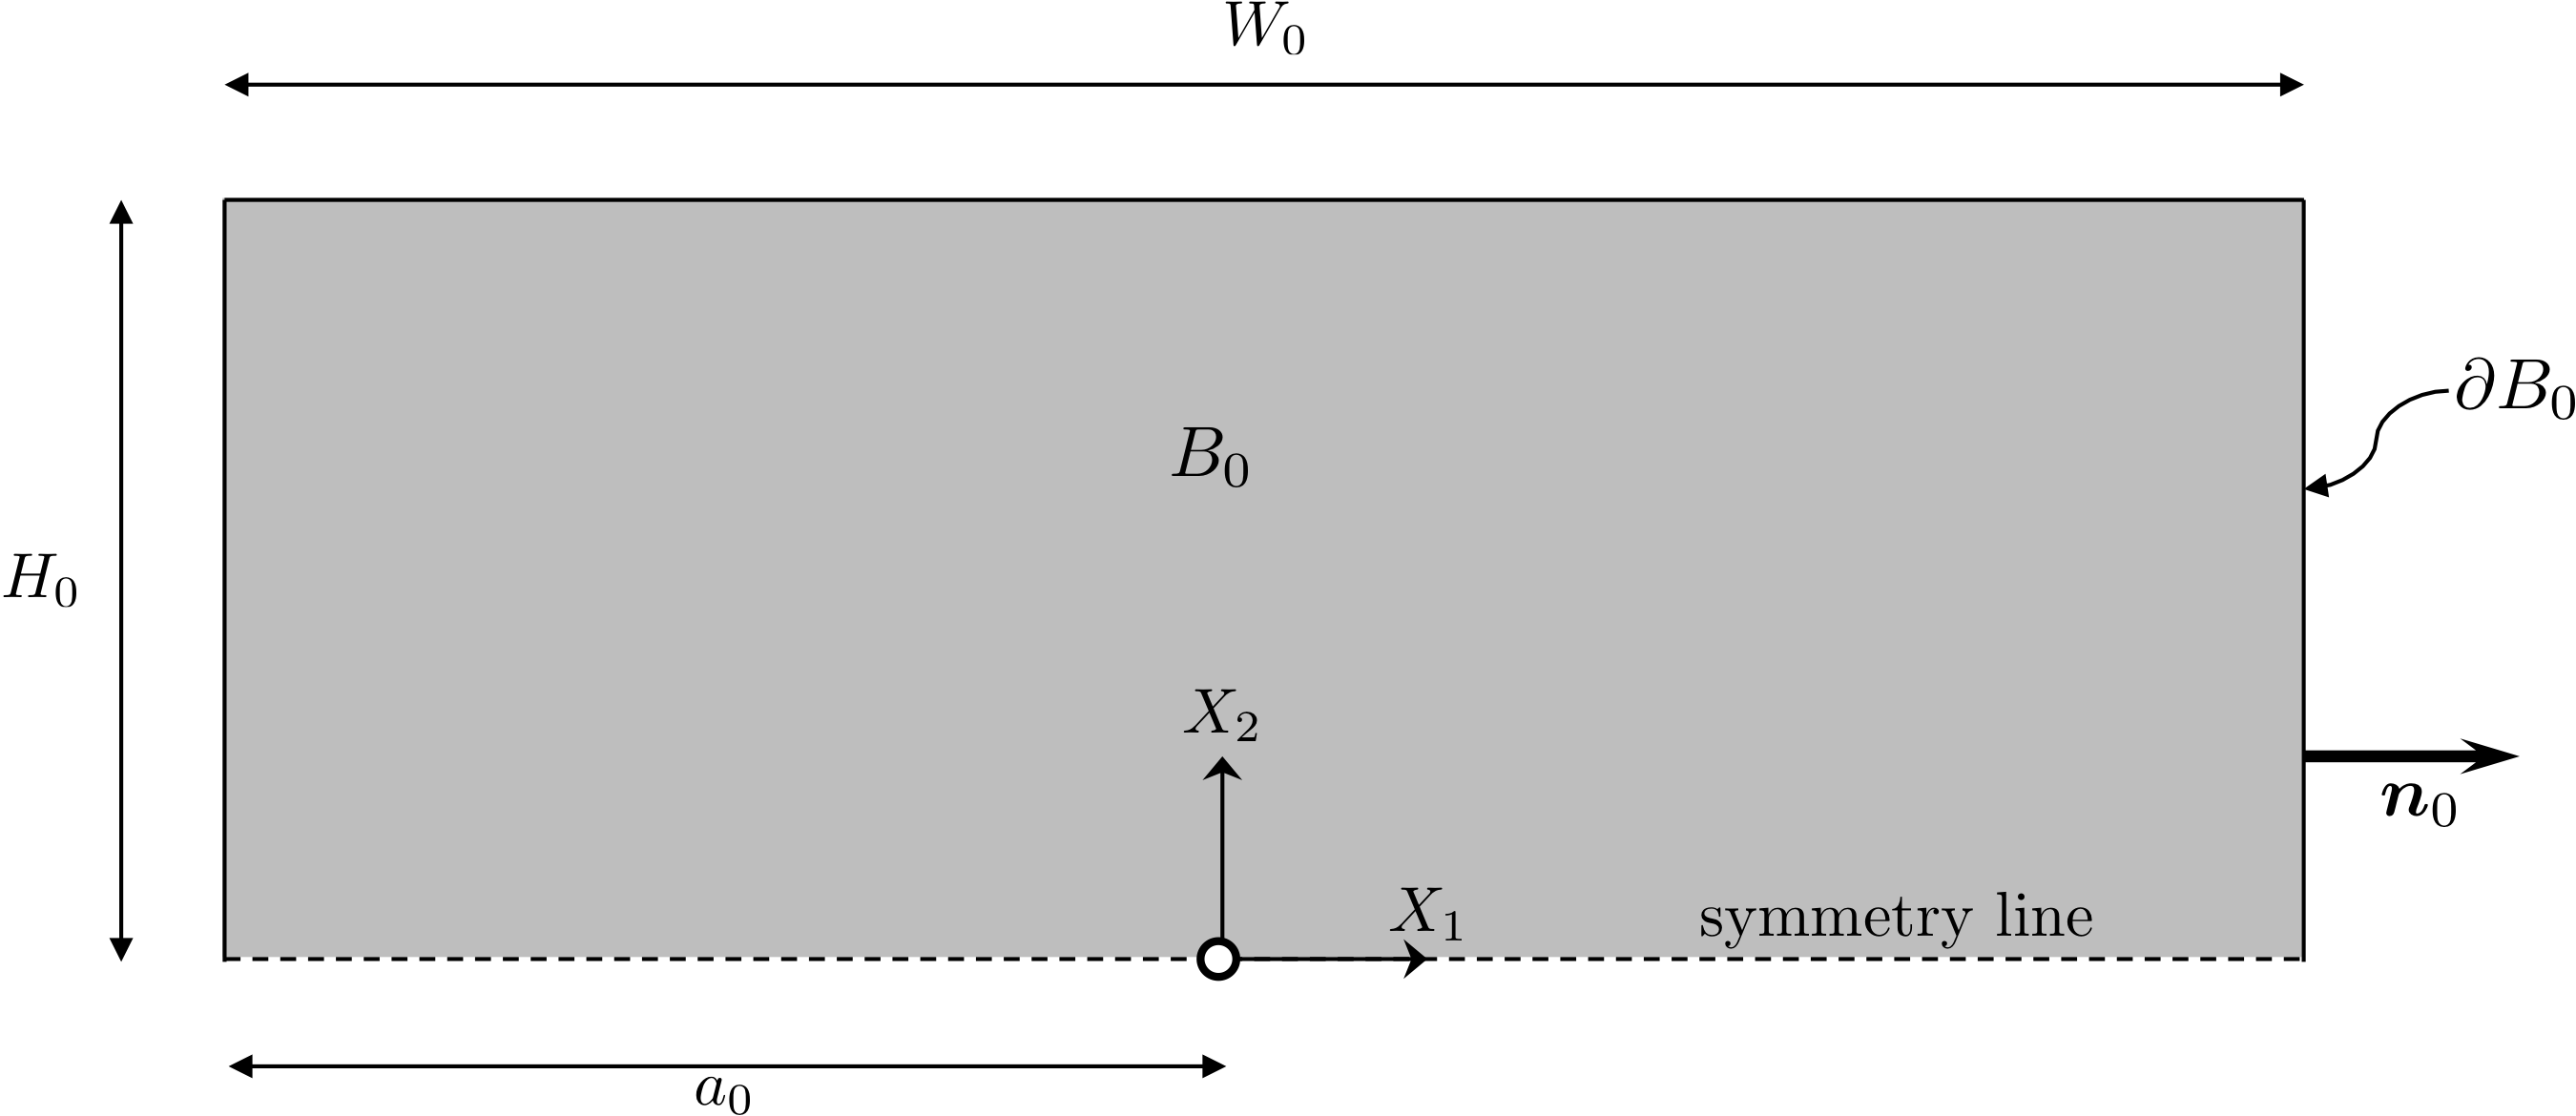
\includegraphics[width=11cm]{Chapter5/figures/JR/domain.png}
  \caption{Schematic of domain for calculations. Actual dimensions are $W_0 = 150 l$, $H_0 = 72 l$, with pre-crack length $a_0 = 0.2 W_0$. Symmetry boundary conditions are applied on the dashed line.}
  \label{fig:domain}
\end{figure}
The adopted values are
\begin{equation}
  \label{eq:domain_size}
  W_0 / l = 150, \quad H_0 / l = 72.
\end{equation}
The origin is placed on the bottom edge, at a distance of $a_0$ from the left-hand side.
The bottom edge is a symmetry plane, which is enforced with the boundary conditions
\begin{equation}
  u_y = 0 \quad \text{on $X_1 > 0, X_2 = 0$}.
\end{equation}
A pre-crack is represented with the boundary condition
\begin{equation}
  \label{eq:phase_bc}
  d = 1 \quad \text{on $ -a_0 \leq X_1 \leq 0, X_2 = 0$},
\end{equation}
thus $a_0$ represents the length of the pre-crack, which will be taken as
\begin{equation}
  \label{eq:pre_crack_length}
  a_0 = 0.2 W_0
\end{equation}
to keep the tip far from the boundary.

On the external boundary $\partial B_0$ (the left, top, and right edges in \Cref{fig:domain}), we drive crack growth by prescribing a displacement field that matches the asymptotic plane strain $K_I$ field solution
\begin{align}
  \label{eq:surfing_bc}
  \begin{Bmatrix}
    \bar{u}_x
    \\
    \bar{u}_y
  \end{Bmatrix}
  = \frac{K_I(t)}{G} \sqrt{\frac{r(t)}{2 \pi}}
  \begin{Bmatrix}
    \left[ 1 - 2\nu + \sin^2 \left( \dfrac{\theta(t)}{2} \right) \right] \cos \left(\dfrac{\theta(t)}{2} \right)
    \\[1em]
    \left[ 2 - 2\nu - \cos^2 \left( \dfrac{\theta(t)}{2} \right) \right] \sin \left(\dfrac{\theta(t)}{2} \right)
  \end{Bmatrix}.
\end{align}
We apply the loading in two stages: in the first, for $0 \leq t \leq 1$, the origin of the $K$-field boundary condition is fixed at the coordinate system origin, where the crack tip sits, and the amplitude of $K_I(t)$ is ramped up linearly; in the second stage $t > 1$, the origin of the $K$-field boundary condition is translated at a constant velocity $v$, while the amplitude of $K_I(t)$ is held fixed, which drives stable crack propagation.
\begin{align}
  r(t)      & =              
  \begin{cases}
    \sqrt{X_1^2 + X_2^2}, \quad t \leqslant 1, \\
    \sqrt{\left( X_1 - v(t-1) \right)^2 + X_2^2}, \quad t > 1,
  \end{cases} \\
  \theta(t) & =              
  \begin{cases}
    \atan(\frac{X_2}{X_1 }), \quad t \leqslant 1, \\
    \atan(\frac{X_2}{X_1 - v(t-1)}), \quad t > 1.
  \end{cases} \\
  K_I(t)    & =              
  \begin{cases}
    t \sqrt{\frac{E G_0}{1 - \nu^2}}, \quad t \leqslant 1, \\
    K_I(t) = \sqrt{\frac{E G_0}{1 - \nu^2}}, \quad t > 1.
  \end{cases}
\end{align}
To monitor the resistance as the crack propagates, the energy release rate $\Gr$ is computed via the $J$-integral on the boundary \citep{rice_path_1968}
\begin{equation}
  \label{eq:J_integral}
  J = \int_{\partial B_0} \bte \cdot \bs{\Sigma} \normal \diff{A},
\end{equation}
where $\bte$ is the unit vector in the direction of crack growth (in our case, the unit vector in the $X_1$-direction), and $\normal_0$ is the unit normal to the boundary.
The symbol $\bs{\Sigma}$ stands for the energy-momentum tensor
\begin{equation}
  \bs{\Sigma} \equiv \psi \bfI - \bfH^T \bfP, \quad \bfH \equiv \defgrad - \bfI,
\end{equation}
The system is always in equilibrium, so we assume $\Gr = J$, that is, that the resistance is always equal to the measured energy release rate.

To construct resistance curves, the other necessary output is the crack extension. The total crack length is computed as
\begin{equation}
  \label{eq:crack_length_definition}
  a = \int_{B_0} \gamma_l \diff{V},
\end{equation}
which is consistent with the fracture energy density \eqref{eq: modified fracture energy}.
The crack extension is given by $\Delta a = a - a_0$.

\begin{figure}[htb!]
  \centering
  \tikzsetnextfilenamesafe{Chapter5/JR/compare_l}
  \begin{tikzpicture}[spy using outlines={rectangle, magnification=3, width=8cm, height=2cm, connect spies}]
    \begin{axis}[
        colormap/jet,
        cycle list={[of colormap,samples of colormap=8]},
        width=\textwidth,
        height=0.45\textwidth,
        xlabel=$\Delta a / r_p$,ylabel=$J / \Gc$,
        xmin=0,
        ymin=0,
        legend style={at={(0.95,0.05)},anchor=south east},
        legend style={nodes={scale=1, transform shape}},
        legend cell align={left},
        every axis plot/.append style={no marks}
      ]
      \addplot table[x expr=(\thisrowno{2}*2-1.7989255734091782)/0.05996418578030594, y expr=\thisrowno{1}*2/2.7, col sep=comma]{Chapter5/data/JR/R_1.csv};
      \addplot table[x expr=(\thisrowno{2}*2-1.6190330160682607)/0.05996418578030594, y expr=\thisrowno{1}*2/2.7, col sep=comma]{Chapter5/data/JR/R_0.9.csv};
      \addplot table[x expr=(\thisrowno{2}*2-1.4391404587273429)/0.05996418578030594, y expr=\thisrowno{1}*2/2.7, col sep=comma]{Chapter5/data/JR/R_0.8.csv};
      \addplot table[x expr=(\thisrowno{2}*2-1.2592479013864248)/0.05996418578030594, y expr=\thisrowno{1}*2/2.7, col sep=comma]{Chapter5/data/JR/R_0.7.csv};
      \addplot table[x expr=(\thisrowno{2}*2-1.079355344045507)/0.05996418578030594, y expr=\thisrowno{1}*2/2.7, col sep=comma]{Chapter5/data/JR/R_0.6.csv};
      \addplot table[x expr=(\thisrowno{2}*2-0.8994627867045891)/0.05996418578030594, y expr=\thisrowno{1}*2/2.7, col sep=comma]{Chapter5/data/JR/R_0.5.csv};
      \addplot table[x expr=(\thisrowno{2}*2-0.7195702293636714)/0.05996418578030594, y expr=\thisrowno{1}*2/2.7, col sep=comma]{Chapter5/data/JR/R_0.4.csv};
      \addplot table[x expr=(\thisrowno{2}*2-0.5396776720227535)/0.05996418578030594, y expr=\thisrowno{1}*2/2.7, col sep=comma]{Chapter5/data/JR/R_0.3.csv};
      \coordinate (spypoint) at (axis cs:30,1.25);
      \coordinate (magnifyglass) at (axis cs:50,0.5);
      \legend{$l/r_p=1$, $l/r_p=0.9$, $l/r_p=0.8$, $l/r_p=0.7$, $l/r_p=0.6$, $l/r_p=0.5$, $l/r_p=0.4$, $l/r_p=0.3$}
    \end{axis}
    \spy [black] on (spypoint) in node[fill=white] at (magnifyglass);
  \end{tikzpicture}
  \caption{J-R curves for different values of $l/r_p$.}
  \label{fig: Chapter5/JR/compare_l}
\end{figure}


Using the E-P-D model with the following set of dimensionless parameters
\begin{align}
  \dfrac{\sigma_y}{E} = 0.005, \quad \dfrac{H}{E} = 0.5, \quad \nu = 0.3, \quad \dfrac{2E\psi_c}{\sigma_y^2} = 1,
\end{align}
the crack growth resistance curves with different values of $l/r_p$ for are plotted in \Cref{fig: Chapter5/JR/compare_l}, where $r_p \equiv \dfrac{1}{3\pi}\dfrac{E\Gc}{(1-\nu^2)\sigma_y^2}$ is the plastic zone size. The results suggest that the resistance curves are remarkably insensitive to $l/r_p$ -- the J-R curves for $l/r_p \leq 0.7$ are virtually indistinguishable. Similar results can be observed with the E-P-PD model. Note that the use of a non-Lorentz-type degradation function, e.g. the quadratic degradation function, results in a strong dependence of the J-R response on the phase-field regularization $l$ \cite{brandon2020cohesive}.
